\documentclass[runningheads]{llncs}

\usepackage[T1]{fontenc}
\usepackage{booktabs}
\usepackage{graphicx}
\usepackage{pgfplots}
\usepackage{xurl}
\pgfplotsset{compat=1.18}
\usepgfplotslibrary{groupplots}

\begin{document}

\title{Understanding Australian and New Zealand Student Visa Approval Rates Through Origin Composition and Weighting}
\titlerunning{Origin Composition and Weighting in AU--NZ Visa Rates}

\author{Vitalii Kaplan\orcidID{0009-0009-8181-2863}}
\authorrunning{V. Kaplan}
\institute{\email{vitalii.v.kaplan@gmail.com}}

\maketitle

\begin{abstract}
According to our previous study, Australia generally had higher recorded student-visa decision approval rates than New Zealand across matched applicant origins. This study tests whether that difference can be accounted for by how decisions are distributed across origins and years. Its main question is whether Australia's higher recorded rate is explained by origins with higher observed Australian rates accounting for larger shares of its decisions. The results do not support that explanation. When Australia and New Zealand were given the same distribution of decisions across origins, Australia had the higher average recorded approval rate. We used aggregate public records for 173 matched origins from 2022--2025. Using the destination-specific origin shares observed in the data, the Australian-minus-New Zealand difference was 5.3 percentage points (95\% confidence interval $-1.4$ to 11.3; $p=0.097$). In a computational comparison that applied the same average origin distribution to both destinations, the standardised rates were 88.5\% for Australia and 77.6\% for New Zealand. The difference therefore increased to 10.9 points (4.2--18.7; $p<0.001$). The composition component was $-5.6$ points ($-14.5$ to $-1.2$; $p=0.005$), confirming that equalising the origin distribution widened rather than removed the estimated difference. The Australian-minus-New Zealand rate component was positive in every year, but its size and the observed gap varied. The distribution of decisions therefore changed the apparent comparison, but it did not account for Australia's higher average recorded rate. These aggregate results do not explain why origin-specific rates differ or identify causal or individual effects.
\keywords{student visas \and Australia \and New Zealand \and administrative data \and origin composition \and temporal comparison \and ISM}
\end{abstract}

\section{Introduction}

International student mobility is now a major form of cross-border movement. UNESCO reported in 2025 that 6.9 million students were studying outside their home countries \cite{UNESCO2025}. Admission to an educational institution, however, is not sufficient for cross-border study: prospective students must also obtain permission to enter and remain in the destination country.

Public visa statistics can reveal how this gateway operates at scale, but cross-national comparisons are not straightforward. Agencies may report applications, completed decisions, or grants, use different origin concepts and study categories, cover different periods, and apply different outcome definitions. A published aggregate approval rate therefore reflects three elements: outcomes recorded within origins, the distribution of decisions across origins, and the administrative population included in the publication. The cross-national data infrastructure used here preserves these distinctions \cite{Kaplan2026CrossNationalDataPaper,Kaplan2026CountryToVisaDataset}.

This article is the third study in a research sequence. It builds on studies of within-New Zealand origin variation and matched Australian--New Zealand decision outcomes \cite{Kaplan2026NZVisaApproval,Kaplan2026AUNZDecisionOutcomes}. The Australian and New Zealand origin-level records overlap for 2022--2025 and permit a common two-outcome decision rate to be calculated, although their published administrative populations are similar rather than identical.

The present study asks whether Australia's higher average recorded rate can be accounted for by how decisions are distributed across origins and years. We compare the recorded difference with a computational condition in which both destinations receive the same average origin distribution while retaining their observed rate for each origin. A symmetric decomposition separates the observed difference into a rate component under shared origin weights and a composition component associated with different origin shares. Supporting analyses examine origin concentration, alternative weights, annual variation, a balanced panel, and a grouped binomial model with origin and year effects. Missing origin--destination--year combinations remain unobserved rather than being converted to zero.

The remainder of the article is organised as follows. Section~2 reviews the relevant literature. Section~3 describes the shared data and the annual structure specific to this study. Section~4 defines the common-weight comparison, decomposition, composition measures, annual analyses, and supporting model. Section~5 presents the results, Section~6 discusses their interpretation, Section~7 states the limitations, and Section~8 concludes by placing the findings within the three-part research sequence.

\section{Literature Review}

International student mobility is structured by relationships between origins and destinations rather than by destination characteristics alone. Bilateral student flows vary with destination income, language, historical ties, migrant networks, and the development level of origin countries \cite{PerkinsNeumayer2014,Weber2023}. Our preceding New Zealand study likewise found that recorded approval rates were associated with origin-level characteristics \cite{Kaplan2026NZVisaApproval}. Comparative evidence from New Zealand and Canada also shows that international students follow heterogeneous temporary and continuing mobility pathways rather than one uniform route to settlement \cite{KingEtAl2024}. These findings establish that the origins represented in a destination are not an interchangeable population. A national summary therefore depends partly on which origins are represented in its student population or administrative records and on the weight attached to each origin.

Visa systems structure unequal access to cross-border mobility \cite{Neumayer2006,Mau2015}. Visa acquisition is also part of a longer pre-departure process that includes information gathering, admission requirements, and documentary preparation \cite{KhanalGaulee2019}. Visa policy can therefore change the population ultimately observed in education and migration statistics. Multi-destination research connects visa-rule changes with enrolment patterns, destination choice, and institutional recruitment \cite{GharibEtAl2026}. In the United States, anticipated visa restrictiveness reduced test taking, score sending to institutions, and enrolment, with larger reductions among students with stronger measured academic achievement \cite{Chen2023}. In Canada, a study-permit reform increased both applications and approval rates for eligible origins, which then increased enrolment \cite{Gonnot2025}. These studies show that visa administration can affect both outcomes and composition. Their policy-specific estimates do not, however, explain descriptive differences between Australian and New Zealand decision records.

The OECD similarly describes international-student populations as products of origin--destination ties, recruitment, admission requirements, institutional gatekeeping, work rights, and post-study opportunities \cite{OECD2022InternationalMigrationOutlook}. It also distinguishes enrolment statistics from permit statistics and documents substantial variation in study-visa rejection rates among reporting countries. This evidence supports explicit treatment of the administrative population and origin distribution. It does not make enrolments, permits, applications, and completed decisions equivalent measures.

Together, this literature establishes that visa administration can shape who reaches enrolment and that origins represented in different destinations are not interchangeable. It does not show how origin shares and annual changes affect comparisons of completed visa decisions. The first study in the present sequence showed that recorded New Zealand approval rates varied across applicant origins and were associated with origin-level characteristics \cite{Kaplan2026NZVisaApproval}. The second found a positive but heterogeneous average Australian--New Zealand difference across matched origins \cite{Kaplan2026AUNZDecisionOutcomes}. This article addresses the remaining measurement question through common weighting and descriptive rate--composition accounting, without attributing the resulting components to particular policies or causal mechanisms.

\section{Data}

This article uses the same aggregate Australian and New Zealand student-visa decision records for 2022--2025 as the preceding matched-origin study. That study documents the original public sources, source verification, population alignment, country-name harmonisation, exclusions, and construction of the pooled comparison \cite{Kaplan2026AUNZDecisionOutcomes}. The underlying source tables are distributed through the Country-to-Visa dataset and documented in its accompanying data paper \cite{Kaplan2026CountryToVisaDataset,Kaplan2026CrossNationalDataPaper}.

The project documentation, preparation and analysis code, final CSV result tables, validation records, run manifests, tests, and publication files are maintained in a public GitHub repository \cite{Kaplan2026UnderstandingAUNZRepository}. Throughout this article, a repository-relative path begins at the root of that repository. The source-retrieval contract at \path{data/README.md} records the required source filenames, snapshot details, published checksums, selective extraction commands, and intended local destinations. Source downloads and extracted inputs under \path{data/original/}, and reproducible prepared and intermediate tables under \path{data/prepared/}, are intentionally not stored in Git. Reviewable final result tables are stored under \path{data/results/}. Their input and output hashes, run configuration, row counts, software versions, and validation status are recorded under \path{data/results/manifests/}. Manuscript-facing selections generated from those verified results are stored under \path{article/tables/} and \path{article/figures/}.

In brief, the New Zealand records report offshore or overseas student-visa decisions by applicant origin. The Australian records cover primary applicants outside Australia in the Higher Education Sector and exclude the separately reported Postgraduate Research Sector. For both destinations, the rate denominator contains completed positive and negative decisions: approvals plus declines in New Zealand and grants plus refusals in Australia. The records are aggregate, and the two administrative populations remain similar rather than identical.

The data preparation specific to this article preserves the origin--destination--year structure needed to study composition and time. Australian financial-year month records were reconstructed into calendar years so that both destinations cover 2022, 2023, 2024, and 2025 on the same annual basis. Destination-specific composition summaries retain every published country origin with a positive decision total. Paired analyses retain an origin only when it has a positive observed total in both destinations at the relevant pooled or annual level. This gives 173 pooled matched origins and 139, 142, 139, and 144 matched origins by year, or 564 matched origin--year pairs. A balanced sensitivity population contains 118 origins observed in both destinations in all four years. Origins absent from one destination are treated as unobserved rather than assigned zero decisions.

\section{Methods}

\subsection{Research Questions and Analytical Rationale}

The main question is whether Australia's higher recorded rate is explained by origins with higher observed Australian rates accounting for larger shares of its decisions. We address it by assigning both destinations the same origin shares while retaining their observed origin-specific rates, then decomposing the observed difference into rate and composition components.

Supporting analyses describe origin concentration and share concordance, compare alternative weighting rules, examine annual and balanced-panel variation, and estimate the destination association after accounting for origin and year. Decision-weighted, origin-weighted, common-weight, decomposition, annual, and model-based estimates are reported separately because they answer different questions. The subsections follow the same order as the Results.

\subsection{Computational Workflow}

The preceding study documents the shared machine-readable analysis contract, outcome notation, validation checks, and construction of pooled and annual long and matched tables \cite{Kaplan2026AUNZDecisionOutcomes}. We use the same two-outcome decision total and define every rate difference as Australia minus New Zealand. The reused tables passed the required schema, count, rate, country-name, period, and reconciliation checks before the present analyses were run.

The extension specific to this article preserves the country--year structure and distinguishes three analytical perspectives. Decision-weighted summaries describe recorded decisions, origin-weighted summaries give each represented origin equal influence, and country--year analyses retain annual origin observations. Destination-specific composition summaries use the long tables, while common-weight, decomposition, and paired annual analyses use the matched tables under the eligibility rules described below. These perspectives answer different questions and are not treated as interchangeable.

\subsection{Missingness and Comparability Gate}

The preceding study documents the shared missingness classifications and comparability gate \cite{Kaplan2026AUNZDecisionOutcomes}. We apply the same rule: paired analyses include an origin only when it has a positive observed decision total in both destinations at the relevant level. Destination-only origins remain in destination-specific summaries, and absence from one source is not interpreted as zero decisions.

For this article, the gate was extended to annual paired analyses, the country--year model, decomposition, and union-based composition distance. The analyses based on observed matched origins were eligible. The union-based distance was not calculated because it would require unsupported zero shares for origins absent from one destination.

\subsection{Same-Origin-Distribution Comparison and Decomposition}

The main analysis used the 173 origins observed in both destinations in the pooled data. We used Kitagawa's symmetric decomposition of the difference between two aggregate rates to separate the contribution of origin-specific rates from the contribution of the distribution of decisions across origins~\cite{Kitagawa1955}. For matched origin $i$ and destination $j$, let $N_{ij}$ be its decision total, $p_{ij}$ its observed approval rate, and $w_{ij}$ its share of all decisions on the matched support:
\[
w_{ij}=\frac{N_{ij}}{\sum_{k}N_{kj}}.
\]
The observed destination rate is $R_j^{\mathrm{obs}}=\sum_i w_{ij}p_{ij}$, and the observed difference is $G^{\mathrm{obs}}=R_{\mathrm{AU}}^{\mathrm{obs}}-R_{\mathrm{NZ}}^{\mathrm{obs}}$. This calculation retains each destination's recorded distribution of decisions across origins.

For the computational same-origin-distribution comparison, both destinations receive the average of their observed matched-support shares, $\bar{w}_i=(w_{i,\mathrm{AU}}+w_{i,\mathrm{NZ}})/2$, while retaining their own observed rate for each origin. The resulting standardised rate is $R_j^{\mathrm{same}}=\sum_i\bar{w}_ip_{ij}$. The Australian-minus-New Zealand difference under these shared weights is the rate component:
\[
C_{\mathrm{rate}}=\sum_i\bar{w}_i(p_{i,\mathrm{AU}}-p_{i,\mathrm{NZ}}).
\]
The symmetric composition component is
\[
C_{\mathrm{composition}}=\sum_i(w_{i,\mathrm{AU}}-w_{i,\mathrm{NZ}})
\frac{p_{i,\mathrm{AU}}+p_{i,\mathrm{NZ}}}{2}.
\]
The two components exactly reconstruct the observed difference, $G^{\mathrm{obs}}=C_{\mathrm{rate}}+C_{\mathrm{composition}}$. They are descriptive accounting quantities and do not identify why the rates or origin distributions differ.

Sensitivity comparisons applied Australian shares, New Zealand shares, and equal weights across origins. The analysis was repeated after requiring at least 20, 50, or 100 decisions for every retained origin in each destination, with threshold zero denoting all origins with positive observed totals. Annual calculations used the 139 to 144 origins observed in both destinations in each year. A balanced sensitivity analysis followed the same origins observed in both destinations in all four years; at threshold zero, this population contained 118 origins.

Uncertainty was estimated with 10,000 paired origin bootstrap resamples~\cite{Efron1979}. Each resample selected matched origins with replacement and recalculated the weights, standardised rates, and decomposition components. Pre-specified deterministic seeds made the pooled, annual, threshold, and balanced analyses reproducible. We report percentile 95\% intervals and supplementary two-sided bootstrap tail p-values around zero with a plus-one correction in each tail.

\subsection{Applicant-Origin Composition}

The composition analysis concerns the distribution of recorded decisions across origins, independently of approval outcomes. For destination $j$, origin $i$ receives share $s_{ij}=N_{ij}/\sum_k N_{kj}$. We report the largest-origin share, combined top-five and top-ten shares, median origin share, Herfindahl--Hirschman Index $\sum_i s_{ij}^2$ on the 0--1 scale, and Gini coefficient for the pooled data and for each year. Ranked-share curves, Lorenz curves, and squares with area proportional to $s_{ij}$ display concentration across the full destination-specific origin sets.

For the 173 matched origins, we calculate Spearman and Pearson correlations between destination shares. Each share retains its full destination total as denominator, so restricting the correlation to matched origins does not renormalise the shares. Spearman's interval uses 10,000 paired bootstrap samples with seed 20260927, while Pearson's interval uses Fisher's $z$ transformation. Correlation measures association rather than equality of shares. The relative-representation plot places each origin at the geometric mean of its two shares on the horizontal axis and at $\log_2(s_{i,\mathrm{AU}}/s_{i,\mathrm{NZ}})$ on the vertical axis. Jensen--Shannon divergence was pre-specified only if absent origins could validly receive zero share and was therefore skipped under the comparability rule in Section~4.3.

\subsection{Temporal Comparison}

The temporal analysis concerns variation across calendar years. For each destination and year from 2022 through 2025, we calculate recorded approvals or grants, declines or refusals, decision totals, represented-origin counts, and the aggregate approval rate. We separately report the median and interquartile range of origin approval rates and the median origin decision total. The aggregate rate is decision-weighted, whereas the median origin rate gives every represented origin equal weight; their annual movements therefore need not coincide.

Annual paired analysis uses only origin--year observations recorded in both destinations. For each year, the Australian rate minus the New Zealand rate is summarised by its mean and $t$-based 95\% interval, median and fixed-seed percentile-bootstrap 95\% interval, quartiles, range, and direction counts. The two-sided Wilcoxon signed-rank test and paired $t$-test follow the same rules as the preceding pooled matched-origin study. Bootstrap medians use 10,000 resamples and a deterministic seed equal to 20260927 plus the calendar year. Annual decomposition follows Section~4.4 on year-specific matched support, with the 118-origin balanced panel used as a sensitivity analysis.

\subsection{Supporting Country--Year Model}

The supporting model asks whether destination remains associated with approval probability after accounting for origin and year. We fit grouped binomial logistic regression to approval and decline counts for origin--year pairs observed in both destinations. The specification contains a destination indicator, origin fixed effects, and year fixed effects. New Zealand is the reference destination, so the destination coefficient is the adjusted log odds for Australia relative to New Zealand.

Origins with the same outcome for all included decisions do not provide a finite fixed-effect estimate~\cite{AlbertAnderson1984}. Twenty-one such origins were excluded before fitting and are listed in the diagnostics. The model uses CR1 sandwich standard errors clustered by origin~\cite{CameronMiller2015}. We report the destination coefficient, Wald interval and test, odds ratio, and standardised predicted probabilities averaged over retained matched origin--year pairs~\cite{MullerMacLehose2014}. The Australian-minus-New Zealand probability contrast uses delta-method uncertainty~\cite{Oehlert1992}.

Diagnostics cover convergence, warnings, separation, non-finite or unusually large estimates, extreme fitted probabilities, influence, and Pearson dispersion. A model is not reported if it fails to converge or retains evidence of unresolved separation. Residual overdispersion is interpreted as unmodelled heterogeneity rather than removed by rescaling the data.

A validated pipeline executed the analyses in dependency order. Reproducibility and output audits recorded file hashes, row counts, random seeds, software versions, warnings, and the producers of publication outputs. A failed blocking check stopped dependent analyses, and every optional output was either produced or skipped with a recorded reason. These controls assess provenance and completeness rather than add substantive findings.

The statistical protocol is recorded at \path{AU_NZ_visa_comparison_methods.md}, and its mapping to executable modules and outputs is documented at \path{src/README.md}. The current article-facing result inventory is recorded at \path{data/results/manifests/minimum_output_checklist.csv}. These paths and all other reader-facing repository paths in this article are stated from the repository root.

\section{Results}

The results first address the main question of whether Australia's higher recorded rate is accounted for by origins with higher observed Australian rates contributing larger shares of its decisions. They then describe the supporting evidence from origin composition, annual variation, and the country--year model. Pooled composition summaries used every origin with positive recorded decisions in each destination. The main comparison used the 173 origins observed in both destinations, while the annual analyses used 139 to 144 matched origins per year. All blocking validation checks passed, pooled counts reconciled with the annual data, and no origin absent from one destination was assigned zero decisions.

\subsection{Main Question: Same-Origin-Distribution Comparison}

Under each destination's observed decision shares within the matched support, the approval rates were 86.7\% for Australia and 81.3\% for New Zealand. The Australian-minus-New Zealand difference was 5.3 percentage points (95\% CI $-1.4$ to 11.3; $p=0.097$). When both destinations were assigned the same average distribution of decisions across origins while retaining their own observed origin-specific rates, the standardised rates were 88.5\% for Australia and 77.6\% for New Zealand. The difference therefore increased to 10.9 points (95\% CI 4.2 to 18.7; $p<0.001$). The difference was also positive under the other common weighting rules: 12.9 points under Australian shares, 9.0 points under New Zealand shares, and 16.3 points when every origin received equal weight (Table~\ref{tab:common-weight-standardisation}). The observed origin distribution therefore did not account for Australia's higher average recorded rate.

The symmetric decomposition gave the same answer from an accounting perspective (Table~\ref{tab:rate-composition-decomposition}). The observed 5.3-point difference was the sum of a positive 10.9-point rate component and a negative 5.6-point composition component (95\% CI $-14.5$ to $-1.2$; $p=0.005$). The negative composition component means that the destination-specific distribution of decisions across origins reduced the observed Australian-minus-New Zealand difference. Applying the same origin distribution to both destinations removed that offset and widened the estimated difference. The decomposition was stable when both destinations were required to have at least 20, 50, or 100 decisions per retained origin. Across these thresholds, the observed difference remained between 5.2 and 5.3 points, the rate component remained 10.9 points, and the composition component ranged from $-5.7$ to $-5.6$ points. These are descriptive accounting quantities, not causal effects.

% Generated by scripts/generate_article_b_decomposition_outputs.py. Do not edit.
\begin{table}
\caption{Pooled approval rates under observed and common applicant-origin weights}
\label{tab:common-weight-standardisation}
\centering
\small
\resizebox{\textwidth}{!}{%
\begin{tabular}{lrrr}
\toprule
Weight distribution & Australia, \% & New Zealand, \% & AU minus NZ, pp (95\% CI); $p$ \\
\midrule
Observed destination-specific weights & 86.7 & 81.3 & 5.3 (-1.4, 11.3); $p=0.097$ \\
Average AU--NZ decision shares & 88.5 & 77.6 & 10.9 (4.2, 18.7); $p<0.001$ \\
Australian decision shares & 86.7 & 73.8 & 12.9 (4.8, 23.3); $p<0.001$ \\
New Zealand decision shares & 90.3 & 81.3 & 9.0 (3.5, 15.3); $p<0.001$ \\
Equal origin weights & 87.8 & 71.5 & 16.3 (12.7, 20.0); $p<0.001$ \\
\bottomrule
\end{tabular}%
}
\parbox{0.96\textwidth}{\scriptsize Notes: All estimates use the 173 origins observed in both destinations. The observed row uses each destination's own decision shares. Common-weight rows apply the same stated origin distribution to both destinations. Bootstrap intervals resample origins. Two-sided bootstrap $p$-values double the smaller empirical tail probability around zero and use a plus-one correction in each tail. pp denotes percentage points.}
\end{table}

\begin{table}
\caption{Symmetric decomposition of the observed Australia--New Zealand aggregate approval-rate difference}
\label{tab:rate-composition-decomposition}
\centering
\small
\resizebox{\textwidth}{!}{%
\begin{tabular}{lrrrr}
\toprule
Period & Origins & Observed gap, pp (95\% CI); $p$ & Rate component, pp (95\% CI); $p$ & Composition component, pp (95\% CI); $p$ \\
\midrule
2022--2025 & 173 & 5.3 (-1.4, 11.3); $p=0.097$ & 10.9 (4.2, 18.7); $p<0.001$ & -5.6 (-14.5, -1.2); $p=0.005$ \\ 
2022 & 139 & -1.7 (-6.6, 3.0); $p=0.525$ & 5.0 (2.1, 8.9); $p=0.002$ & -6.7 (-12.5, -1.4); $p<0.001$ \\
2023 & 142 & 0.6 (-6.5, 5.0); $p=0.746$ & 8.9 (4.5, 15.9); $p<0.001$ & -8.4 (-19.3, -2.7); $p<0.001$ \\
2024 & 139 & 11.9 (-0.9, 20.6); $p=0.066$ & 13.5 (4.3, 24.0); $p<0.001$ & -1.5 (-13.6, 2.4); $p=0.520$ \\
2025 & 144 & 6.3 (0.4, 14.3); $p=0.032$ & 9.2 (0.9, 18.9); $p=0.022$ & -2.9 (-8.6, 0.5); $p=0.111$ \\
\bottomrule
\end{tabular}%
}
\parbox{0.96\textwidth}{\scriptsize Notes: Values are percentage points. The rate component applies average AU--NZ origin shares to origin-specific rate differences. The composition component applies decision-share differences to average origin-specific rates. Their sum reproduces the observed matched-support gap. Two-sided bootstrap $p$-values double the smaller empirical tail probability around zero and use a plus-one correction in each tail. Components are descriptive accounting quantities, not causal effects.}
\end{table}


\subsection{Supporting Result: Applicant-Origin Composition}

Recorded decisions were more concentrated across applicant origins in Australia than in New Zealand. Across 2022--2025, Australia's largest origin accounted for 32.1\% of decisions, compared with 23.8\% in New Zealand. The top five origins accounted for 73.4\% and 58.2\%, respectively, while the top ten accounted for 85.9\% and 75.1\%. Australia's HHI was 0.177 and its Gini coefficient was 0.947, compared with 0.111 and 0.901 for New Zealand (Table~\ref{tab:origin-composition}). The annual results showed the same broader pattern. Australia's top five origins contributed 72.2\% to 75.4\% of decisions each year, compared with 56.1\% to 60.7\% in New Zealand, and Australia's annual HHI exceeded New Zealand's in every year (Table~\ref{tab:annual-origin-composition}). The ranked-share and Lorenz curves show that the difference extended across the distributions rather than arising only from the largest origin (Figure~\ref{fig:origin-composition-curves}). The equal-area proportional-square display provides an additional view of this pattern. Australia's total area was concentrated in fewer large origin squares, while New Zealand distributed the same total area across a longer sequence of medium and small squares (Figure~\ref{fig:origin-share-squares}). Nevertheless, the ordering of matched-origin shares was similar across destinations. Spearman correlation was 0.858 (bootstrap 95\% CI 0.805 to 0.896; $p<0.001$), and Pearson correlation was 0.952 (95\% CI 0.936 to 0.965; $p<0.001$). Figure~\ref{fig:relative-origin-representation} shows the relative representation of each matched origin directly. Origins above zero contributed a larger share of Australian decisions, while origins below zero contributed a larger share of New Zealand decisions. A union-based composition distance was not calculated because origins absent from one destination could not be interpreted as having zero decisions.

% Generated by scripts/generate_article_model_composition_outputs.py. Do not edit.
\begin{table}
\caption{Applicant-origin composition and concentration of recorded decisions, 2022--2025}
\label{tab:origin-composition}
\centering
\small
\begin{tabular*}{\textwidth}{@{\extracolsep{\fill}}lrrrrrr@{}}
\toprule
Destination & Origins & Top 1 & Top 5 & Top 10 & HHI & Gini \\
\midrule
Australia & 192 & 32.1\% & 73.4\% & 85.9\% & 0.177 & 0.947 \\
New Zealand & 179 & 23.8\% & 58.2\% & 75.1\% & 0.111 & 0.901 \\
\bottomrule
\end{tabular*}
\vspace{0.4em}
\begin{tabular*}{\textwidth}{@{\extracolsep{\fill}}lrrr@{}}
\toprule
Matched-share measure & Coefficient & 95\% CI & Two-sided $p$ \\
\midrule
Spearman & 0.858 & [0.805, 0.896] & $p<0.001$ \\
Pearson & 0.952 & [0.936, 0.965] & $p<0.001$ \\
\bottomrule
\end{tabular*}
\parbox{0.96\textwidth}{\scriptsize Notes: Shares use each destination's complete recorded decision total. HHI is on the 0--1 scale. Jensen--Shannon divergence was not calculated because the missingness audit did not permit absent origins to be assigned zero.}
\end{table}

% Generated by scripts/generate_decomposition_outputs.py. Do not edit.
\begin{table}
\caption{Annual applicant-origin concentration}
\label{tab:annual-origin-composition}
\centering
\small
\begin{tabular*}{\textwidth}{@{\extracolsep{\fill}}llrrrrr@{}}
\toprule
Year & Destination & Origins & Top 1, \% & Top 5, \% & HHI & Gini \\
\midrule
2022 & Australia & 164 & 28.1 & 72.2 & 0.159 & 0.931 \\
2022 & New Zealand & 149 & 29.8 & 57.1 & 0.122 & 0.880 \\
2023 & Australia & 167 & 28.3 & 75.4 & 0.177 & 0.945 \\
2023 & New Zealand & 157 & 23.3 & 59.6 & 0.114 & 0.890 \\
2024 & Australia & 162 & 39.1 & 74.7 & 0.211 & 0.942 \\
2024 & New Zealand & 151 & 22.9 & 60.7 & 0.117 & 0.892 \\
2025 & Australia & 171 & 33.5 & 74.8 & 0.177 & 0.939 \\
2025 & New Zealand & 155 & 23.7 & 56.1 & 0.102 & 0.884 \\
\bottomrule
\end{tabular*}
\parbox{0.96\textwidth}{\scriptsize Notes: Shares use all positive recorded decisions represented for the stated destination and year. HHI is reported on the 0--1 scale.}
\end{table}


\begin{figure}
\centering
% Generated by scripts/generate_article_model_composition_outputs.py. Do not edit.
\begin{minipage}[t]{0.48\textwidth}
\centering
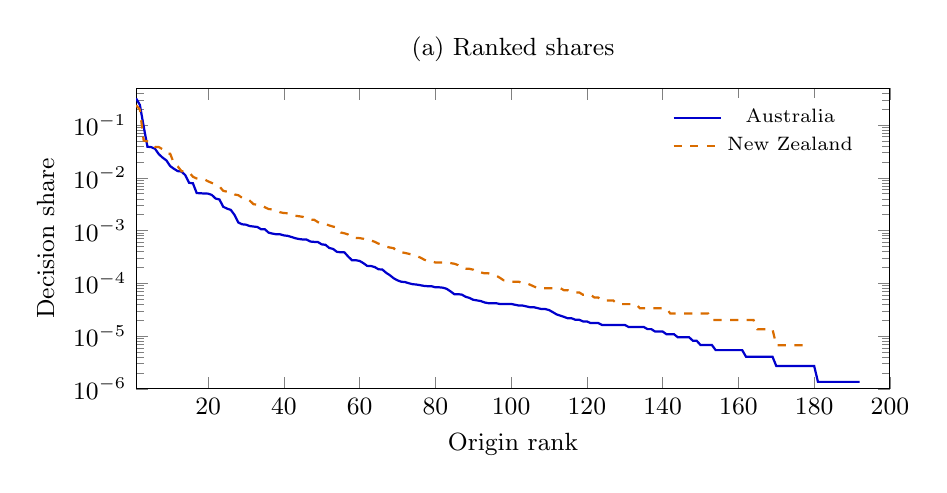
\begin{tikzpicture}
\begin{semilogyaxis}[width=0.92\linewidth,height=5.4cm,xmin=1,xmax=200,ymin=0.000001,ymax=0.5,xlabel={Origin rank},ylabel={Decision share},title={(a) Ranked shares},legend style={font=\scriptsize,at={{(0.97,0.97)}},anchor=north east,draw=none},tick label style={font=\small},label style={font=\small},title style={font=\small}]
\addplot[blue!80!black,thick] coordinates {(1,0.321051389703) (2,0.240936015101) (3,0.0945494044132) (4,0.0388460370153) (5,0.0381612206817) (6,0.0354748421532) (7,0.0280856061099) (8,0.0241367245981) (9,0.0213784742563) (10,0.0166823971013) (11,0.0148001692378) (12,0.0133979908438) (13,0.0131362689579) (14,0.0112025103604) (15,0.00803337021849) (16,0.00788013408839) (17,0.00514086875393) (18,0.0051001865955) (19,0.00503238299811) (20,0.00501746620669) (21,0.00473133502571) (22,0.00404516262015) (23,0.00388650220226) (24,0.00282876608301) (25,0.00261043849943) (26,0.00246805094491) (27,0.00197172861203) (28,0.00142116340125) (29,0.00131538978932) (30,0.00129369263816) (31,0.00121910868103) (32,0.00119198724208) (33,0.00117029009091) (34,0.00106044826314) (35,0.0010563800473) (36,0.000912636420838) (37,0.000876022478249) (38,0.000851613183189) (39,0.000850257111241) (40,0.000810931024756) (41,0.000794658161383) (42,0.000756688146846) (43,0.000717362060361) (44,0.000691596693354) (45,0.000678035973877) (46,0.000675323829981) (47,0.000619724880123) (48,0.000610232376489) (49,0.000606164160646) (50,0.000547853066892) (51,0.00053700449131) (52,0.000467844821975) (53,0.000448859814706) (54,0.000395973008744) (55,0.000387836577057) (56,0.00038648050511) (57,0.000321389051618) (58,0.000273926533446) (59,0.000273926533446) (60,0.00026579010176) (61,0.0002413808067) (62,0.000214259367745) (63,0.000212903295797) (64,0.000203410792163) (65,0.000184425784894) (66,0.000183069712947) (67,0.000158660417887) (68,0.000142387554514) (69,0.000124758619193) (70,0.000113910043611) (71,0.000107129683873) (72,0.000105773611925) (73,0.000100349324134) (74,9.62811082905e-05) (75,9.49250363427e-05) (76,9.22128924472e-05) (77,8.95007485517e-05) (78,8.8144676604e-05) (79,8.8144676604e-05) (80,8.40764607607e-05) (81,8.40764607607e-05) (82,8.27203888129e-05) (83,7.86521729697e-05) (84,7.05157412832e-05) (85,6.23793095966e-05) (86,6.23793095966e-05) (87,6.10232376489e-05) (88,5.55989498579e-05) (89,5.28868059624e-05) (90,4.88185901191e-05) (91,4.74625181714e-05) (92,4.61064462236e-05) (93,4.33943023281e-05) (94,4.20382303804e-05) (95,4.20382303804e-05) (96,4.20382303804e-05) (97,4.06821584326e-05) (98,4.06821584326e-05) (99,4.06821584326e-05) (100,4.06821584326e-05) (101,3.93260864848e-05) (102,3.79700145371e-05) (103,3.79700145371e-05) (104,3.66139425893e-05) (105,3.52578706416e-05) (106,3.52578706416e-05) (107,3.39017986938e-05) (108,3.25457267461e-05) (109,3.25457267461e-05) (110,3.11896547983e-05) (111,2.84775109028e-05) (112,2.57653670073e-05) (113,2.44092950596e-05) (114,2.30532231118e-05) (115,2.16971511641e-05) (116,2.16971511641e-05) (117,2.03410792163e-05) (118,2.03410792163e-05) (119,1.89850072685e-05) (120,1.89850072685e-05) (121,1.76289353208e-05) (122,1.76289353208e-05) (123,1.76289353208e-05) (124,1.6272863373e-05) (125,1.6272863373e-05) (126,1.6272863373e-05) (127,1.6272863373e-05) (128,1.6272863373e-05) (129,1.6272863373e-05) (130,1.6272863373e-05) (131,1.49167914253e-05) (132,1.49167914253e-05) (133,1.49167914253e-05) (134,1.49167914253e-05) (135,1.49167914253e-05) (136,1.35607194775e-05) (137,1.35607194775e-05) (138,1.22046475298e-05) (139,1.22046475298e-05) (140,1.22046475298e-05) (141,1.0848575582e-05) (142,1.0848575582e-05) (143,1.0848575582e-05) (144,9.49250363427e-06) (145,9.49250363427e-06) (146,9.49250363427e-06) (147,9.49250363427e-06) (148,8.13643168652e-06) (149,8.13643168652e-06) (150,6.78035973877e-06) (151,6.78035973877e-06) (152,6.78035973877e-06) (153,6.78035973877e-06) (154,5.42428779101e-06) (155,5.42428779101e-06) (156,5.42428779101e-06) (157,5.42428779101e-06) (158,5.42428779101e-06) (159,5.42428779101e-06) (160,5.42428779101e-06) (161,5.42428779101e-06) (162,4.06821584326e-06) (163,4.06821584326e-06) (164,4.06821584326e-06) (165,4.06821584326e-06) (166,4.06821584326e-06) (167,4.06821584326e-06) (168,4.06821584326e-06) (169,4.06821584326e-06) (170,2.71214389551e-06) (171,2.71214389551e-06) (172,2.71214389551e-06) (173,2.71214389551e-06) (174,2.71214389551e-06) (175,2.71214389551e-06) (176,2.71214389551e-06) (177,2.71214389551e-06) (178,2.71214389551e-06) (179,2.71214389551e-06) (180,2.71214389551e-06) (181,1.35607194775e-06) (182,1.35607194775e-06) (183,1.35607194775e-06) (184,1.35607194775e-06) (185,1.35607194775e-06) (186,1.35607194775e-06) (187,1.35607194775e-06) (188,1.35607194775e-06) (189,1.35607194775e-06) (190,1.35607194775e-06) (191,1.35607194775e-06) (192,1.35607194775e-06)};\addlegendentry{Australia}
\addplot[orange!85!black,thick,dashed] coordinates {(1,0.238473639627) (2,0.197470856359) (3,0.050999690748) (4,0.0490567813588) (5,0.0458096352171) (6,0.038441369852) (7,0.0383069124548) (8,0.0347034542105) (9,0.0290293520498) (10,0.0285856426391) (11,0.018790421255) (12,0.0164508625442) (13,0.0133247280599) (14,0.0133247280599) (15,0.0128003442109) (16,0.01046750837) (17,0.0097145469458) (18,0.00939184919258) (19,0.00936495771315) (20,0.00858510480954) (21,0.00800021513184) (22,0.0073548196254) (23,0.00688421873529) (24,0.00566065642101) (25,0.00546569319511) (26,0.00537157301709) (27,0.00483374342839) (28,0.00467911742164) (29,0.0041816250521) (30,0.00414801070281) (31,0.00369757842228) (32,0.00315974883358) (33,0.003092520135) (34,0.00304546004598) (35,0.00276982238178) (36,0.0025546905463) (37,0.00253452193672) (38,0.00242023314913) (39,0.00222526992322) (40,0.00215131835478) (41,0.0021311497452) (42,0.00199669234803) (43,0.00190929503987) (44,0.00186895782071) (45,0.0018218977317) (46,0.00169416320439) (47,0.00161348876608) (48,0.00160676589623) (49,0.00144541701962) (50,0.0013512968416) (51,0.00133112823202) (52,0.00125045379372) (53,0.00118994796499) (54,0.00114961074584) (55,0.00092103317064) (56,0.000887418821346) (57,0.000840358732336) (58,0.000732792814597) (59,0.000726069944738) (60,0.000719347074879) (61,0.000699178465303) (62,0.000658841246151) (63,0.000652118376292) (64,0.00061178115714) (65,0.00056472106813) (66,0.000537829588695) (67,0.000497492369543) (68,0.000477323759967) (69,0.000463878020249) (70,0.000396649321662) (71,0.000389926451804) (72,0.000376480712086) (73,0.000363034972369) (74,0.000349589232652) (75,0.000329420623076) (76,0.0003092520135) (77,0.000282360534065) (78,0.000262191924489) (79,0.000262191924489) (80,0.000248746184771) (81,0.000248746184771) (82,0.000248746184771) (83,0.000248746184771) (84,0.000242023314913) (85,0.000235300445054) (86,0.000221854705337) (87,0.000194963225902) (88,0.000188240356043) (89,0.000188240356043) (90,0.000181517486185) (91,0.000161348876608) (92,0.000161348876608) (93,0.00015462600675) (94,0.00015462600675) (95,0.000147903136891) (96,0.000141180267032) (97,0.000127734527315) (98,0.000114288787598) (99,0.000114288787598) (100,0.000107565917739) (101,0.000107565917739) (102,0.000107565917739) (103,0.00010084304788) (104,0.00010084304788) (105,9.41201780216e-05) (106,8.73973081629e-05) (107,8.06744383042e-05) (108,8.06744383042e-05) (109,8.06744383042e-05) (110,8.06744383042e-05) (111,8.06744383042e-05) (112,8.06744383042e-05) (113,8.06744383042e-05) (114,7.39515684455e-05) (115,7.39515684455e-05) (116,6.72286985869e-05) (117,6.72286985869e-05) (118,6.72286985869e-05) (119,6.05058287282e-05) (120,6.05058287282e-05) (121,6.05058287282e-05) (122,5.37829588695e-05) (123,5.37829588695e-05) (124,4.70600890108e-05) (125,4.70600890108e-05) (126,4.70600890108e-05) (127,4.70600890108e-05) (128,4.03372191521e-05) (129,4.03372191521e-05) (130,4.03372191521e-05) (131,4.03372191521e-05) (132,4.03372191521e-05) (133,4.03372191521e-05) (134,3.36143492934e-05) (135,3.36143492934e-05) (136,3.36143492934e-05) (137,3.36143492934e-05) (138,3.36143492934e-05) (139,3.36143492934e-05) (140,3.36143492934e-05) (141,3.36143492934e-05) (142,2.68914794347e-05) (143,2.68914794347e-05) (144,2.68914794347e-05) (145,2.68914794347e-05) (146,2.68914794347e-05) (147,2.68914794347e-05) (148,2.68914794347e-05) (149,2.68914794347e-05) (150,2.68914794347e-05) (151,2.68914794347e-05) (152,2.68914794347e-05) (153,2.01686095761e-05) (154,2.01686095761e-05) (155,2.01686095761e-05) (156,2.01686095761e-05) (157,2.01686095761e-05) (158,2.01686095761e-05) (159,2.01686095761e-05) (160,2.01686095761e-05) (161,2.01686095761e-05) (162,2.01686095761e-05) (163,2.01686095761e-05) (164,2.01686095761e-05) (165,1.34457397174e-05) (166,1.34457397174e-05) (167,1.34457397174e-05) (168,1.34457397174e-05) (169,1.34457397174e-05) (170,6.72286985869e-06) (171,6.72286985869e-06) (172,6.72286985869e-06) (173,6.72286985869e-06) (174,6.72286985869e-06) (175,6.72286985869e-06) (176,6.72286985869e-06) (177,6.72286985869e-06) (178,6.72286985869e-06) (179,6.72286985869e-06)};\addlegendentry{New Zealand}
\end{semilogyaxis}
\end{tikzpicture}
\end{minipage}%
\hfill
\begin{minipage}[t]{0.48\textwidth}
\centering
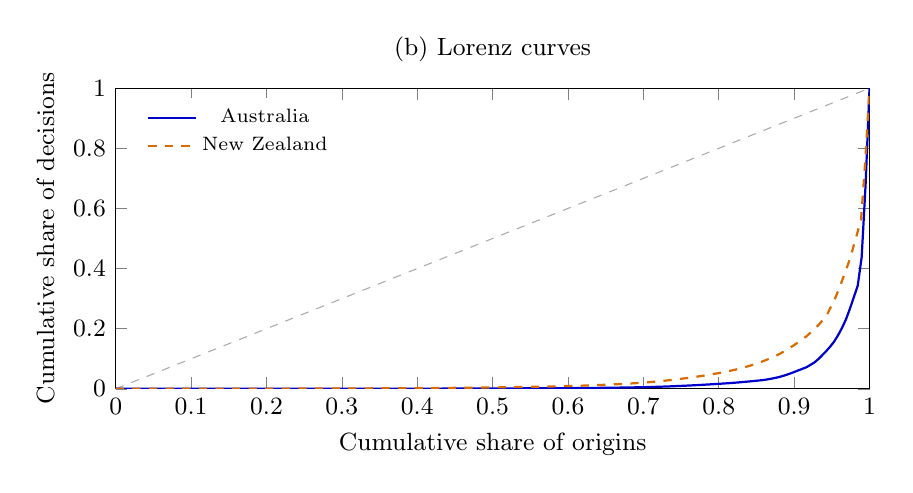
\begin{tikzpicture}
\begin{axis}[width=0.92\linewidth,height=5.4cm,xmin=0,xmax=1,ymin=0,ymax=1,xlabel={Cumulative share of origins},ylabel={Cumulative share of decisions},title={(b) Lorenz curves},legend style={font=\scriptsize,at={{(0.03,0.97)}},anchor=north west,draw=none},tick label style={font=\small},label style={font=\small},title style={font=\small}]
\addplot[gray!65,dashed,domain=0:1,forget plot] {x};
\addplot[blue!80!black,thick] coordinates {(0,0) (0.00520833333333,1.35607194775e-06) (0.0104166666667,2.71214389551e-06) (0.015625,4.06821584326e-06) (0.0208333333333,5.42428779101e-06) (0.0260416666667,6.78035973877e-06) (0.03125,8.13643168652e-06) (0.0364583333333,9.49250363427e-06) (0.0416666666667,1.0848575582e-05) (0.046875,1.22046475298e-05) (0.0520833333333,1.35607194775e-05) (0.0572916666667,1.49167914253e-05) (0.0625,1.6272863373e-05) (0.0677083333333,1.89850072685e-05) (0.0729166666667,2.16971511641e-05) (0.078125,2.44092950596e-05) (0.0833333333333,2.71214389551e-05) (0.0885416666667,2.98335828506e-05) (0.09375,3.25457267461e-05) (0.0989583333333,3.52578706416e-05) (0.104166666667,3.79700145371e-05) (0.109375,4.06821584326e-05) (0.114583333333,4.33943023281e-05) (0.119791666667,4.61064462236e-05) (0.125,5.01746620669e-05) (0.130208333333,5.42428779101e-05) (0.135416666667,5.83110937534e-05) (0.140625,6.23793095966e-05) (0.145833333333,6.64475254399e-05) (0.151041666667,7.05157412832e-05) (0.15625,7.45839571264e-05) (0.161458333333,7.86521729697e-05) (0.166666666667,8.40764607607e-05) (0.171875,8.95007485517e-05) (0.177083333333,9.49250363427e-05) (0.182291666667,0.000100349324134) (0.1875,0.000105773611925) (0.192708333333,0.000111197899716) (0.197916666667,0.000116622187507) (0.203125,0.000122046475298) (0.208333333333,0.000128826835037) (0.213541666667,0.000135607194775) (0.21875,0.000142387554514) (0.223958333333,0.000149167914253) (0.229166666667,0.000157304345939) (0.234375,0.000165440777626) (0.239583333333,0.00017493328126) (0.244791666667,0.000184425784894) (0.25,0.000193918288529) (0.255208333333,0.000203410792163) (0.260416666667,0.000214259367745) (0.265625,0.000225107943327) (0.270833333333,0.000235956518909) (0.276041666667,0.000248161166439) (0.28125,0.000260365813969) (0.286458333333,0.000272570461498) (0.291666666667,0.000286131180976) (0.296875,0.000299691900453) (0.302083333333,0.000314608691879) (0.307291666667,0.000329525483304) (0.3125,0.000344442274729) (0.317708333333,0.000359359066155) (0.322916666667,0.00037427585758) (0.328125,0.000390548720953) (0.333333333333,0.000406821584326) (0.338541666667,0.000423094447699) (0.34375,0.000439367311072) (0.348958333333,0.000455640174445) (0.354166666667,0.000471913037818) (0.359375,0.000488185901191) (0.364583333333,0.000505814836512) (0.369791666667,0.000523443771833) (0.375,0.000541072707154) (0.380208333333,0.000560057714422) (0.385416666667,0.000579042721691) (0.390625,0.000599383800907) (0.395833333333,0.000619724880123) (0.401041666667,0.000641422031287) (0.40625,0.000663119182451) (0.411458333333,0.000686172405563) (0.416666666667,0.000710581700623) (0.421875,0.00073634706763) (0.427083333333,0.000764824578533) (0.432291666667,0.000796014233331) (0.4375,0.000828559960077) (0.442708333333,0.000861105686823) (0.447916666667,0.000895007485517) (0.453125,0.000930265356159) (0.458333333333,0.0009655232268) (0.463541666667,0.00100213716939) (0.46875,0.00104010718393) (0.473958333333,0.00107807719846) (0.479166666667,0.00111740328495) (0.484375,0.00115808544338) (0.489583333333,0.00119876760181) (0.494791666667,0.00123944976025) (0.5,0.00128013191868) (0.505208333333,0.00132217014906) (0.510416666667,0.00136420837944) (0.515625,0.00140624660982) (0.520833333333,0.00144964091215) (0.526041666667,0.00149574735837) (0.53125,0.00154320987654) (0.536458333333,0.00159202846666) (0.541666666667,0.00164491527262) (0.546875,0.00170051422248) (0.552083333333,0.00176153746013) (0.557291666667,0.00182391676973) (0.5625,0.00188629607932) (0.567708333333,0.00195681182061) (0.572916666667,0.00203546399358) (0.578125,0.00211818438239) (0.583333333333,0.00220226084315) (0.588541666667,0.00228633730391) (0.59375,0.00237448198052) (0.598958333333,0.00246262665712) (0.604166666667,0.00255212740567) (0.609375,0.00264434029812) (0.614583333333,0.00273926533446) (0.619791666667,0.00283554644275) (0.625,0.00293589576689) (0.630208333333,0.00304166937881) (0.635416666667,0.00314879906268) (0.640625,0.00326270910629) (0.645833333333,0.00338746772549) (0.651041666667,0.00352985528) (0.65625,0.00368851569789) (0.661458333333,0.00387158541084) (0.666666666667,0.00405601119573) (0.671875,0.00425942198789) (0.677083333333,0.00447232528369) (0.682291666667,0.00468658465144) (0.6875,0.00492796545814) (0.692708333333,0.00519375555989) (0.697916666667,0.00546768209334) (0.703125,0.00574160862679) (0.708333333333,0.0060629976784) (0.713541666667,0.00644947818351) (0.71875,0.00683731476057) (0.723958333333,0.00723328776932) (0.729166666667,0.00768214758402) (0.734375,0.008149992406) (0.739583333333,0.00868699689731) (0.744791666667,0.0092348499642) (0.75,0.00984101412485) (0.755208333333,0.0104512465013) (0.760416666667,0.0110709713815) (0.765625,0.0117462952114) (0.770833333333,0.0124243311853) (0.776041666667,0.0131159278787) (0.78125,0.013833289939) (0.786458333333,0.0145899780859) (0.791666666667,0.0153846362473) (0.796875,0.016195567272) (0.802083333333,0.0170458243833) (0.807291666667,0.0178974375664) (0.8125,0.0187734600447) (0.817708333333,0.0196860964655) (0.822916666667,0.0207424765128) (0.828125,0.021802924776) (0.833333333333,0.0229732148669) (0.838541666667,0.024165202109) (0.84375,0.02538431079) (0.848958333333,0.0266780034281) (0.854166666667,0.0279933932175) (0.859375,0.0294145566187) (0.864583333333,0.0313862852307) (0.869791666667,0.0338543361757) (0.875,0.0364647746751) (0.880208333333,0.0392935407581) (0.885416666667,0.0431800429604) (0.890625,0.0472252055805) (0.895833333333,0.0519565406062) (0.901041666667,0.0569740068129) (0.90625,0.062006389811) (0.911458333333,0.0671065764065) (0.916666666667,0.0722474451605) (0.921875,0.0801275792488) (0.927083333333,0.0881609494673) (0.932291666667,0.0993634598277) (0.9375,0.112499728786) (0.942708333333,0.125897719629) (0.947916666667,0.140697888867) (0.953125,0.157380285968) (0.958333333333,0.178758760225) (0.963541666667,0.202895484823) (0.96875,0.230981090933) (0.973958333333,0.266455933086) (0.979166666667,0.304617153768) (0.984375,0.343463190783) (0.989583333333,0.438012595196) (0.994791666667,0.678948610297) (1,1)};\addlegendentry{Australia}
\addplot[orange!85!black,thick,dashed] coordinates {(0,0) (0.00558659217877,6.72286985869e-06) (0.0111731843575,1.34457397174e-05) (0.0167597765363,2.01686095761e-05) (0.0223463687151,2.68914794347e-05) (0.0279329608939,3.36143492934e-05) (0.0335195530726,4.03372191521e-05) (0.0391061452514,4.70600890108e-05) (0.0446927374302,5.37829588695e-05) (0.0502793296089,6.05058287282e-05) (0.0558659217877,6.72286985869e-05) (0.0614525139665,8.06744383042e-05) (0.0670391061453,9.41201780216e-05) (0.072625698324,0.000107565917739) (0.0782122905028,0.000121011657456) (0.0837988826816,0.000134457397174) (0.0893854748603,0.00015462600675) (0.0949720670391,0.000174794616326) (0.100558659218,0.000194963225902) (0.106145251397,0.000215131835478) (0.111731843575,0.000235300445054) (0.117318435754,0.00025546905463) (0.122905027933,0.000275637664206) (0.128491620112,0.000295806273782) (0.134078212291,0.000315974883358) (0.139664804469,0.000336143492934) (0.145251396648,0.00035631210251) (0.150837988827,0.000376480712086) (0.156424581006,0.000403372191521) (0.162011173184,0.000430263670956) (0.167597765363,0.000457155150391) (0.173184357542,0.000484046629825) (0.178770949721,0.00051093810926) (0.184357541899,0.000537829588695) (0.189944134078,0.00056472106813) (0.195530726257,0.000591612547564) (0.201117318436,0.000618504026999) (0.206703910615,0.000645395506434) (0.212290502793,0.000672286985869) (0.217877094972,0.000705901335162) (0.223463687151,0.000739515684455) (0.22905027933,0.000773130033749) (0.234636871508,0.000806744383042) (0.240223463687,0.000840358732336) (0.245810055866,0.000873973081629) (0.251396648045,0.000907587430923) (0.256983240223,0.000941201780216) (0.262569832402,0.000981538999368) (0.268156424581,0.00102187621852) (0.27374301676,0.00106221343767) (0.279329608939,0.00110255065682) (0.284916201117,0.00114288787598) (0.290502793296,0.00118322509513) (0.296089385475,0.00123028518414) (0.301675977654,0.00127734527315) (0.307262569832,0.00132440536216) (0.312849162011,0.00137146545117) (0.31843575419,0.00142524841004) (0.324022346369,0.00147903136891) (0.329608938547,0.00153953719764) (0.335195530726,0.00160004302637) (0.340782122905,0.0016605488551) (0.346368715084,0.00172777755368) (0.351955307263,0.00179500625227) (0.357541899441,0.00186223495086) (0.36312849162,0.0019361865193) (0.368715083799,0.00201013808775) (0.374301675978,0.00209081252605) (0.379888268156,0.00217148696436) (0.385474860335,0.00225216140266) (0.391061452514,0.00233283584096) (0.396648044693,0.00241351027927) (0.402234636872,0.00249418471757) (0.40782122905,0.00257485915588) (0.413407821229,0.00266225646404) (0.418994413408,0.00275637664206) (0.424581005587,0.00285721968994) (0.430167597765,0.00295806273782) (0.435754189944,0.00306562865556) (0.441340782123,0.0031731945733) (0.446927374302,0.00328076049104) (0.45251396648,0.00339504927864) (0.458100558659,0.00350933806623) (0.463687150838,0.00363707259355) (0.469273743017,0.00377825286058) (0.474860335196,0.00392615599747) (0.480446927374,0.00408078200422) (0.486033519553,0.00423540801097) (0.491620111732,0.00439675688758) (0.497206703911,0.00455810576419) (0.502793296089,0.00473962325037) (0.508379888268,0.00492786360642) (0.513966480447,0.00511610396246) (0.519553072626,0.00531106718836) (0.525139664804,0.0055329218937) (0.530726256983,0.00576822233875) (0.536312849162,0.00601024565366) (0.541899441341,0.00625899183844) (0.54748603352,0.00650773802321) (0.553072625698,0.00675648420798) (0.558659217877,0.00700523039275) (0.564245810056,0.00726742231724) (0.569832402235,0.00752961424173) (0.575418994413,0.00781197477579) (0.581005586592,0.00812122678929) (0.586592178771,0.00845064741237) (0.59217877095,0.00880023664502) (0.597765363128,0.00916327161739) (0.603351955307,0.00953975232947) (0.608938547486,0.00992967878128) (0.614525139665,0.0103263281029) (0.620111731844,0.0107902061232) (0.625698324022,0.0112675298832) (0.631284916201,0.0117650222527) (0.63687150838,0.0123028518414) (0.642458100559,0.0128675729095) (0.648044692737,0.0134793540667) (0.653631284916,0.014131472443) (0.659217877095,0.0147903136891) (0.664804469274,0.0154894921544) (0.670391061453,0.0162088392293) (0.675977653631,0.016934909174) (0.68156424581,0.0176677019886) (0.687150837989,0.018508060721) (0.692737430168,0.0193954795423) (0.698324022346,0.0203165127129) (0.703910614525,0.0214661234588) (0.709497206704,0.0226560714238) (0.715083798883,0.0239065252175) (0.720670391061,0.0252376534495) (0.72625698324,0.0265889502911) (0.731843575419,0.0280343673107) (0.737430167598,0.0296411332069) (0.743016759777,0.031254621973) (0.748603351955,0.0329487851774) (0.754189944134,0.0347706829091) (0.759776536313,0.0366396407298) (0.765363128492,0.0385489357697) (0.77094972067,0.0405456281177) (0.776536312849,0.0426767778629) (0.782122905028,0.0448280962177) (0.787709497207,0.0470533661409) (0.793296089385,0.0494735992901) (0.798882681564,0.0520081212268) (0.804469273743,0.0545628117731) (0.810055865922,0.0573326341549) (0.815642458101,0.0603780942009) (0.821229050279,0.0634706143358) (0.826815642458,0.0666303631694) (0.832402234637,0.0703279415917) (0.837988826816,0.0744759522945) (0.843575418994,0.0786575773466) (0.849162011173,0.0833366947683) (0.854748603352,0.0881704381967) (0.860335195531,0.0935420112137) (0.865921787709,0.0990077044089) (0.871508379888,0.10466836083) (0.877094972067,0.111552579565) (0.882681564246,0.118907399191) (0.888268156425,0.126907614322) (0.893854748603,0.135492719132) (0.899441340782,0.144857676845) (0.905027932961,0.154249526038) (0.91061452514,0.163964072983) (0.916201117318,0.174431581353) (0.921787709497,0.187231925564) (0.927374301676,0.200556653624) (0.932960893855,0.213881381684) (0.938547486034,0.230332244228) (0.944134078212,0.249122665483) (0.949720670391,0.277708308123) (0.95530726257,0.306737660172) (0.960893854749,0.341441114383) (0.966480446927,0.379748026838) (0.972067039106,0.41818939669) (0.977653631285,0.463999031907) (0.983240223464,0.513055813266) (0.988826815642,0.564055504014) (0.994413407821,0.761526360373) (1,1)};\addlegendentry{New Zealand}
\end{axis}
\end{tikzpicture}
\end{minipage}

\caption{Distribution of recorded decision shares across applicant origins, 2022--2025. Panel (a) ranks each destination's observed origins and uses a logarithmic share axis. Panel (b) gives Lorenz curves. The diagonal denotes equal shares across origins.}
\label{fig:origin-composition-curves}
\end{figure}

\begin{figure}
\centering
% Generated by scripts/generate_proportional_share_squares.py. Do not edit.
% Every square has side sqrt(origin share / largest origin share), so its area
% is proportional to that origin's share of its destination's decisions.
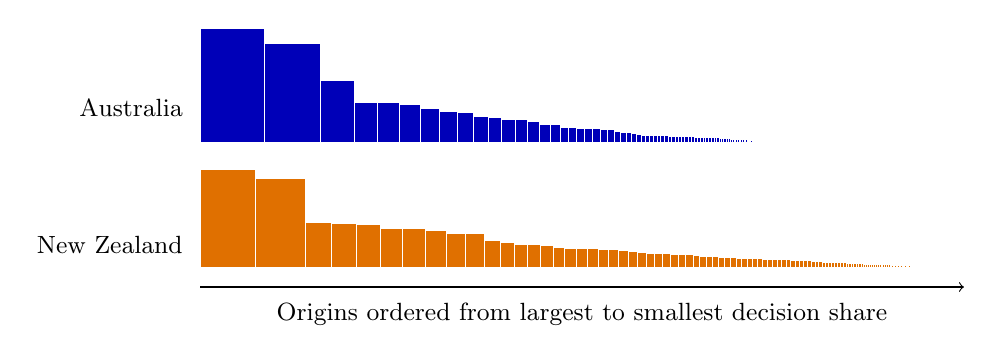
\begin{tikzpicture}[x={0.80\textwidth/11.920458577},y=1.45cm]
\node[font=\small,anchor=east] at (-0.12,1.65) {Australia};
\node[font=\small,anchor=east] at (-0.12,0.45) {New Zealand};
\filldraw[fill=blue!72!black,draw=white,line width=0.12pt] (0.000000000,1.350000000) rectangle (1.000000000,2.350000000);
\filldraw[fill=blue!72!black,draw=white,line width=0.12pt] (1.000000000,1.350000000) rectangle (1.866290565,2.216290565);
\filldraw[fill=blue!72!black,draw=white,line width=0.12pt] (1.866290565,1.350000000) rectangle (2.408968448,1.892677882);
\filldraw[fill=blue!72!black,draw=white,line width=0.12pt] (2.408968448,1.350000000) rectangle (2.756813702,1.697845254);
\filldraw[fill=blue!72!black,draw=white,line width=0.12pt] (2.756813702,1.350000000) rectangle (3.101579243,1.694765541);
\filldraw[fill=blue!72!black,draw=white,line width=0.12pt] (3.101579243,1.350000000) rectangle (3.433988385,1.682409142);
\filldraw[fill=blue!72!black,draw=white,line width=0.12pt] (3.433988385,1.350000000) rectangle (3.729758727,1.645770342);
\filldraw[fill=blue!72!black,draw=white,line width=0.12pt] (3.729758727,1.350000000) rectangle (4.003948903,1.624190176);
\filldraw[fill=blue!72!black,draw=white,line width=0.12pt] (4.003948903,1.350000000) rectangle (4.261997247,1.608048344);
\filldraw[fill=blue!72!black,draw=white,line width=0.12pt] (4.261997247,1.350000000) rectangle (4.489948482,1.577951235);
\filldraw[fill=blue!72!black,draw=white,line width=0.12pt] (4.489948482,1.350000000) rectangle (4.704655413,1.564706931);
\filldraw[fill=blue!72!black,draw=white,line width=0.12pt] (4.704655413,1.350000000) rectangle (4.908938570,1.554283157);
\filldraw[fill=blue!72!black,draw=white,line width=0.12pt] (4.908938570,1.350000000) rectangle (5.111216611,1.552278041);
\filldraw[fill=blue!72!black,draw=white,line width=0.12pt] (5.111216611,1.350000000) rectangle (5.298013827,1.536797216);
\filldraw[fill=blue!72!black,draw=white,line width=0.12pt] (5.298013827,1.350000000) rectangle (5.456197485,1.508183658);
\filldraw[fill=blue!72!black,draw=white,line width=0.12pt] (5.456197485,1.350000000) rectangle (5.612865206,1.506667721);
\filldraw[fill=blue!72!black,draw=white,line width=0.12pt] (5.612865206,1.350000000) rectangle (5.739406125,1.476540918);
\filldraw[fill=blue!72!black,draw=white,line width=0.12pt] (5.739406125,1.350000000) rectangle (5.865445359,1.476039234);
\filldraw[fill=blue!72!black,draw=white,line width=0.12pt] (5.865445359,1.350000000) rectangle (5.990643986,1.475198627);
\filldraw[fill=blue!72!black,draw=white,line width=0.12pt] (5.990643986,1.350000000) rectangle (6.115656921,1.475012935);
\filldraw[fill=blue!72!black,draw=white,line width=0.12pt] (6.115656921,1.350000000) rectangle (6.237052976,1.471396055);
\filldraw[fill=blue!72!black,draw=white,line width=0.12pt] (6.237052976,1.350000000) rectangle (6.349301519,1.462248544);
\filldraw[fill=blue!72!black,draw=white,line width=0.12pt] (6.349301519,1.350000000) rectangle (6.459326723,1.460025204);
\filldraw[fill=blue!72!black,draw=white,line width=0.12pt] (6.459326723,1.350000000) rectangle (6.553193356,1.443866633);
\filldraw[fill=blue!72!black,draw=white,line width=0.12pt] (6.553193356,1.350000000) rectangle (6.643364890,1.440171534);
\filldraw[fill=blue!72!black,draw=white,line width=0.12pt] (6.643364890,1.350000000) rectangle (6.731042718,1.437677828);
\filldraw[fill=blue!72!black,draw=white,line width=0.12pt] (6.731042718,1.350000000) rectangle (6.809410272,1.428367554);
\filldraw[fill=blue!72!black,draw=white,line width=0.12pt] (6.809410272,1.350000000) rectangle (6.875942908,1.416532636);
\filldraw[fill=blue!72!black,draw=white,line width=0.12pt] (6.875942908,1.350000000) rectangle (6.939951748,1.414008840);
\filldraw[fill=blue!72!black,draw=white,line width=0.12pt] (6.939951748,1.350000000) rectangle (7.003430485,1.413478737);
\filldraw[fill=blue!72!black,draw=white,line width=0.12pt] (7.003430485,1.350000000) rectangle (7.065052222,1.411621737);
\filldraw[fill=blue!72!black,draw=white,line width=0.12pt] (7.065052222,1.350000000) rectangle (7.125984656,1.410932434);
\filldraw[fill=blue!72!black,draw=white,line width=0.12pt] (7.125984656,1.350000000) rectangle (7.186359981,1.410375326);
\filldraw[fill=blue!72!black,draw=white,line width=0.12pt] (7.186359981,1.350000000) rectangle (7.243832134,1.407472153);
\filldraw[fill=blue!72!black,draw=white,line width=0.12pt] (7.243832134,1.350000000) rectangle (7.301193940,1.407361806);
\filldraw[fill=blue!72!black,draw=white,line width=0.12pt] (7.301193940,1.350000000) rectangle (7.354510439,1.403316499);
\filldraw[fill=blue!72!black,draw=white,line width=0.12pt] (7.354510439,1.350000000) rectangle (7.406746491,1.402236052);
\filldraw[fill=blue!72!black,draw=white,line width=0.12pt] (7.406746491,1.350000000) rectangle (7.458249655,1.401503164);
\filldraw[fill=blue!72!black,draw=white,line width=0.12pt] (7.458249655,1.350000000) rectangle (7.509711798,1.401462142);
\filldraw[fill=blue!72!black,draw=white,line width=0.12pt] (7.509711798,1.350000000) rectangle (7.559969737,1.400257940);
\filldraw[fill=blue!72!black,draw=white,line width=0.12pt] (7.559969737,1.350000000) rectangle (7.609720861,1.399751124);
\filldraw[fill=blue!72!black,draw=white,line width=0.12pt] (7.609720861,1.350000000) rectangle (7.658268844,1.398547983);
\filldraw[fill=blue!72!black,draw=white,line width=0.12pt] (7.658268844,1.350000000) rectangle (7.705538444,1.397269600);
\filldraw[fill=blue!72!black,draw=white,line width=0.12pt] (7.705538444,1.350000000) rectangle (7.751951394,1.396412950);
\filldraw[fill=blue!72!black,draw=white,line width=0.12pt] (7.751951394,1.350000000) rectangle (7.797907063,1.395955669);
\filldraw[fill=blue!72!black,draw=white,line width=0.12pt] (7.797907063,1.350000000) rectangle (7.843770728,1.395863665);
\filldraw[fill=blue!72!black,draw=white,line width=0.12pt] (7.843770728,1.350000000) rectangle (7.887705886,1.393935158);
\filldraw[fill=blue!72!black,draw=white,line width=0.12pt] (7.887705886,1.350000000) rectangle (7.931303261,1.393597375);
\filldraw[fill=blue!72!black,draw=white,line width=0.12pt] (7.931303261,1.350000000) rectangle (7.974755069,1.393451808);
\filldraw[fill=blue!72!black,draw=white,line width=0.12pt] (7.974755069,1.350000000) rectangle (8.016064078,1.391309009);
\filldraw[fill=blue!72!black,draw=white,line width=0.12pt] (8.016064078,1.350000000) rectangle (8.056962041,1.390897963);
\filldraw[fill=blue!72!black,draw=white,line width=0.12pt] (8.056962041,1.350000000) rectangle (8.095135687,1.388173646);
\filldraw[fill=blue!72!black,draw=white,line width=0.12pt] (8.095135687,1.350000000) rectangle (8.132526773,1.387391087);
\filldraw[fill=blue!72!black,draw=white,line width=0.12pt] (8.132526773,1.350000000) rectangle (8.167646046,1.385119273);
\filldraw[fill=blue!72!black,draw=white,line width=0.12pt] (8.167646046,1.350000000) rectangle (8.202402632,1.384756586);
\filldraw[fill=blue!72!black,draw=white,line width=0.12pt] (8.202402632,1.350000000) rectangle (8.237098401,1.384695769);
\filldraw[fill=blue!72!black,draw=white,line width=0.12pt] (8.237098401,1.350000000) rectangle (8.268737803,1.381639402);
\filldraw[fill=blue!72!black,draw=white,line width=0.12pt] (8.268737803,1.350000000) rectangle (8.297947683,1.379209880);
\filldraw[fill=blue!72!black,draw=white,line width=0.12pt] (8.297947683,1.350000000) rectangle (8.327157563,1.379209880);
\filldraw[fill=blue!72!black,draw=white,line width=0.12pt] (8.327157563,1.350000000) rectangle (8.355930363,1.378772800);
\filldraw[fill=blue!72!black,draw=white,line width=0.12pt] (8.355930363,1.350000000) rectangle (8.383350150,1.377419788);
\filldraw[fill=blue!72!black,draw=white,line width=0.12pt] (8.383350150,1.350000000) rectangle (8.409183614,1.375833463);
\filldraw[fill=blue!72!black,draw=white,line width=0.12pt] (8.409183614,1.350000000) rectangle (8.434935196,1.375751582);
\filldraw[fill=blue!72!black,draw=white,line width=0.12pt] (8.434935196,1.350000000) rectangle (8.460106152,1.375170956);
\filldraw[fill=blue!72!black,draw=white,line width=0.12pt] (8.460106152,1.350000000) rectangle (8.484073697,1.373967545);
\filldraw[fill=blue!72!black,draw=white,line width=0.12pt] (8.484073697,1.350000000) rectangle (8.507952963,1.373879266);
\filldraw[fill=blue!72!black,draw=white,line width=0.12pt] (8.507952963,1.350000000) rectangle (8.530183350,1.372230387);
\filldraw[fill=blue!72!black,draw=white,line width=0.12pt] (8.530183350,1.350000000) rectangle (8.551242883,1.371059533);
\filldraw[fill=blue!72!black,draw=white,line width=0.12pt] (8.551242883,1.350000000) rectangle (8.570955668,1.369712786);
\filldraw[fill=blue!72!black,draw=white,line width=0.12pt] (8.570955668,1.350000000) rectangle (8.589791887,1.368836219);
\filldraw[fill=blue!72!black,draw=white,line width=0.12pt] (8.589791887,1.350000000) rectangle (8.608058905,1.368267017);
\filldraw[fill=blue!72!black,draw=white,line width=0.12pt] (8.608058905,1.350000000) rectangle (8.626209939,1.368151035);
\filldraw[fill=blue!72!black,draw=white,line width=0.12pt] (8.626209939,1.350000000) rectangle (8.643889438,1.367679499);
\filldraw[fill=blue!72!black,draw=white,line width=0.12pt] (8.643889438,1.350000000) rectangle (8.661206861,1.367317423);
\filldraw[fill=blue!72!black,draw=white,line width=0.12pt] (8.661206861,1.350000000) rectangle (8.678401898,1.367195037);
\filldraw[fill=blue!72!black,draw=white,line width=0.12pt] (8.678401898,1.350000000) rectangle (8.695349511,1.366947613);
\filldraw[fill=blue!72!black,draw=white,line width=0.12pt] (8.695349511,1.350000000) rectangle (8.712046035,1.366696524);
\filldraw[fill=blue!72!black,draw=white,line width=0.12pt] (8.712046035,1.350000000) rectangle (8.728615587,1.366569552);
\filldraw[fill=blue!72!black,draw=white,line width=0.12pt] (8.728615587,1.350000000) rectangle (8.745185139,1.366569552);
\filldraw[fill=blue!72!black,draw=white,line width=0.12pt] (8.745185139,1.350000000) rectangle (8.761367800,1.366182661);
\filldraw[fill=blue!72!black,draw=white,line width=0.12pt] (8.761367800,1.350000000) rectangle (8.777550461,1.366182661);
\filldraw[fill=blue!72!black,draw=white,line width=0.12pt] (8.777550461,1.350000000) rectangle (8.793602086,1.366051625);
\filldraw[fill=blue!72!black,draw=white,line width=0.12pt] (8.793602086,1.350000000) rectangle (8.809254022,1.365651937);
\filldraw[fill=blue!72!black,draw=white,line width=0.12pt] (8.809254022,1.350000000) rectangle (8.824074280,1.364820258);
\filldraw[fill=blue!72!black,draw=white,line width=0.12pt] (8.824074280,1.350000000) rectangle (8.838013325,1.363939045);
\filldraw[fill=blue!72!black,draw=white,line width=0.12pt] (8.838013325,1.350000000) rectangle (8.851952369,1.363939045);
\filldraw[fill=blue!72!black,draw=white,line width=0.12pt] (8.851952369,1.350000000) rectangle (8.865739070,1.363786701);
\filldraw[fill=blue!72!black,draw=white,line width=0.12pt] (8.865739070,1.350000000) rectangle (8.878898771,1.363159701);
\filldraw[fill=blue!72!black,draw=white,line width=0.12pt] (8.878898771,1.350000000) rectangle (8.891733491,1.362834720);
\filldraw[fill=blue!72!black,draw=white,line width=0.12pt] (8.891733491,1.350000000) rectangle (8.904064691,1.362331200);
\filldraw[fill=blue!72!black,draw=white,line width=0.12pt] (8.904064691,1.350000000) rectangle (8.916223418,1.362158727);
\filldraw[fill=blue!72!black,draw=white,line width=0.12pt] (8.916223418,1.350000000) rectangle (8.928207190,1.361983772);
\filldraw[fill=blue!72!black,draw=white,line width=0.12pt] (8.928207190,1.350000000) rectangle (8.939833157,1.361625967);
\filldraw[fill=blue!72!black,draw=white,line width=0.12pt] (8.939833157,1.350000000) rectangle (8.951276026,1.361442869);
\filldraw[fill=blue!72!black,draw=white,line width=0.12pt] (8.951276026,1.350000000) rectangle (8.962718895,1.361442869);
\filldraw[fill=blue!72!black,draw=white,line width=0.12pt] (8.962718895,1.350000000) rectangle (8.974161765,1.361442869);
\filldraw[fill=blue!72!black,draw=white,line width=0.12pt] (8.974161765,1.350000000) rectangle (8.985418559,1.361256794);
\filldraw[fill=blue!72!black,draw=white,line width=0.12pt] (8.985418559,1.350000000) rectangle (8.996675352,1.361256794);
\filldraw[fill=blue!72!black,draw=white,line width=0.12pt] (8.996675352,1.350000000) rectangle (9.007932146,1.361256794);
\filldraw[fill=blue!72!black,draw=white,line width=0.12pt] (9.007932146,1.350000000) rectangle (9.019188940,1.361256794);
\filldraw[fill=blue!72!black,draw=white,line width=0.12pt] (9.019188940,1.350000000) rectangle (9.030256531,1.361067591);
\filldraw[fill=blue!72!black,draw=white,line width=0.12pt] (9.030256531,1.350000000) rectangle (9.041131627,1.360875096);
\filldraw[fill=blue!72!black,draw=white,line width=0.12pt] (9.041131627,1.350000000) rectangle (9.052006723,1.360875096);
\filldraw[fill=blue!72!black,draw=white,line width=0.12pt] (9.052006723,1.350000000) rectangle (9.062685856,1.360679132);
\filldraw[fill=blue!72!black,draw=white,line width=0.12pt] (9.062685856,1.350000000) rectangle (9.073165361,1.360479505);
\filldraw[fill=blue!72!black,draw=white,line width=0.12pt] (9.073165361,1.350000000) rectangle (9.083644865,1.360479505);
\filldraw[fill=blue!72!black,draw=white,line width=0.12pt] (9.083644865,1.350000000) rectangle (9.093920865,1.360276000);
\filldraw[fill=blue!72!black,draw=white,line width=0.12pt] (9.093920865,1.350000000) rectangle (9.103989248,1.360068383);
\filldraw[fill=blue!72!black,draw=white,line width=0.12pt] (9.103989248,1.350000000) rectangle (9.114057630,1.360068383);
\filldraw[fill=blue!72!black,draw=white,line width=0.12pt] (9.114057630,1.350000000) rectangle (9.123914023,1.359856393);
\filldraw[fill=blue!72!black,draw=white,line width=0.12pt] (9.123914023,1.350000000) rectangle (9.133332133,1.359418110);
\filldraw[fill=blue!72!black,draw=white,line width=0.12pt] (9.133332133,1.350000000) rectangle (9.142290542,1.358958409);
\filldraw[fill=blue!72!black,draw=white,line width=0.12pt] (9.142290542,1.350000000) rectangle (9.151010017,1.358719475);
\filldraw[fill=blue!72!black,draw=white,line width=0.12pt] (9.151010017,1.350000000) rectangle (9.159483824,1.358473807);
\filldraw[fill=blue!72!black,draw=white,line width=0.12pt] (9.159483824,1.350000000) rectangle (9.167704624,1.358220800);
\filldraw[fill=blue!72!black,draw=white,line width=0.12pt] (9.167704624,1.350000000) rectangle (9.175925424,1.358220800);
\filldraw[fill=blue!72!black,draw=white,line width=0.12pt] (9.175925424,1.350000000) rectangle (9.183885179,1.357959755);
\filldraw[fill=blue!72!black,draw=white,line width=0.12pt] (9.183885179,1.350000000) rectangle (9.191844934,1.357959755);
\filldraw[fill=blue!72!black,draw=white,line width=0.12pt] (9.191844934,1.350000000) rectangle (9.199534788,1.357689854);
\filldraw[fill=blue!72!black,draw=white,line width=0.12pt] (9.199534788,1.350000000) rectangle (9.207224643,1.357689854);
\filldraw[fill=blue!72!black,draw=white,line width=0.12pt] (9.207224643,1.350000000) rectangle (9.214634772,1.357410129);
\filldraw[fill=blue!72!black,draw=white,line width=0.12pt] (9.214634772,1.350000000) rectangle (9.222044901,1.357410129);
\filldraw[fill=blue!72!black,draw=white,line width=0.12pt] (9.222044901,1.350000000) rectangle (9.229455030,1.357410129);
\filldraw[fill=blue!72!black,draw=white,line width=0.12pt] (9.229455030,1.350000000) rectangle (9.236574451,1.357119422);
\filldraw[fill=blue!72!black,draw=white,line width=0.12pt] (9.236574451,1.350000000) rectangle (9.243693873,1.357119422);
\filldraw[fill=blue!72!black,draw=white,line width=0.12pt] (9.243693873,1.350000000) rectangle (9.250813294,1.357119422);
\filldraw[fill=blue!72!black,draw=white,line width=0.12pt] (9.250813294,1.350000000) rectangle (9.257932716,1.357119422);
\filldraw[fill=blue!72!black,draw=white,line width=0.12pt] (9.257932716,1.350000000) rectangle (9.265052138,1.357119422);
\filldraw[fill=blue!72!black,draw=white,line width=0.12pt] (9.265052138,1.350000000) rectangle (9.272171559,1.357119422);
\filldraw[fill=blue!72!black,draw=white,line width=0.12pt] (9.272171559,1.350000000) rectangle (9.279290981,1.357119422);
\filldraw[fill=blue!72!black,draw=white,line width=0.12pt] (9.279290981,1.350000000) rectangle (9.286107308,1.356816327);
\filldraw[fill=blue!72!black,draw=white,line width=0.12pt] (9.286107308,1.350000000) rectangle (9.292923635,1.356816327);
\filldraw[fill=blue!72!black,draw=white,line width=0.12pt] (9.292923635,1.350000000) rectangle (9.299739962,1.356816327);
\filldraw[fill=blue!72!black,draw=white,line width=0.12pt] (9.299739962,1.350000000) rectangle (9.306556290,1.356816327);
\filldraw[fill=blue!72!black,draw=white,line width=0.12pt] (9.306556290,1.350000000) rectangle (9.313372617,1.356816327);
\filldraw[fill=blue!72!black,draw=white,line width=0.12pt] (9.313372617,1.350000000) rectangle (9.319871730,1.356499113);
\filldraw[fill=blue!72!black,draw=white,line width=0.12pt] (9.319871730,1.350000000) rectangle (9.326370843,1.356499113);
\filldraw[fill=blue!72!black,draw=white,line width=0.12pt] (9.326370843,1.350000000) rectangle (9.332536443,1.356165600);
\filldraw[fill=blue!72!black,draw=white,line width=0.12pt] (9.332536443,1.350000000) rectangle (9.338702043,1.356165600);
\filldraw[fill=blue!72!black,draw=white,line width=0.12pt] (9.338702043,1.350000000) rectangle (9.344867643,1.356165600);
\filldraw[fill=blue!72!black,draw=white,line width=0.12pt] (9.344867643,1.350000000) rectangle (9.350680626,1.355812983);
\filldraw[fill=blue!72!black,draw=white,line width=0.12pt] (9.350680626,1.350000000) rectangle (9.356493610,1.355812983);
\filldraw[fill=blue!72!black,draw=white,line width=0.12pt] (9.356493610,1.350000000) rectangle (9.362306593,1.355812983);
\filldraw[fill=blue!72!black,draw=white,line width=0.12pt] (9.362306593,1.350000000) rectangle (9.367744141,1.355437548);
\filldraw[fill=blue!72!black,draw=white,line width=0.12pt] (9.367744141,1.350000000) rectangle (9.373181689,1.355437548);
\filldraw[fill=blue!72!black,draw=white,line width=0.12pt] (9.373181689,1.350000000) rectangle (9.378619237,1.355437548);
\filldraw[fill=blue!72!black,draw=white,line width=0.12pt] (9.378619237,1.350000000) rectangle (9.384056785,1.355437548);
\filldraw[fill=blue!72!black,draw=white,line width=0.12pt] (9.384056785,1.350000000) rectangle (9.389090977,1.355034191);
\filldraw[fill=blue!72!black,draw=white,line width=0.12pt] (9.389090977,1.350000000) rectangle (9.394125168,1.355034191);
\filldraw[fill=blue!72!black,draw=white,line width=0.12pt] (9.394125168,1.350000000) rectangle (9.398720735,1.354595567);
\filldraw[fill=blue!72!black,draw=white,line width=0.12pt] (9.398720735,1.350000000) rectangle (9.403316302,1.354595567);
\filldraw[fill=blue!72!black,draw=white,line width=0.12pt] (9.403316302,1.350000000) rectangle (9.407911869,1.354595567);
\filldraw[fill=blue!72!black,draw=white,line width=0.12pt] (9.407911869,1.350000000) rectangle (9.412507435,1.354595567);
\filldraw[fill=blue!72!black,draw=white,line width=0.12pt] (9.412507435,1.350000000) rectangle (9.416617835,1.354110400);
\filldraw[fill=blue!72!black,draw=white,line width=0.12pt] (9.416617835,1.350000000) rectangle (9.420728235,1.354110400);
\filldraw[fill=blue!72!black,draw=white,line width=0.12pt] (9.420728235,1.350000000) rectangle (9.424838635,1.354110400);
\filldraw[fill=blue!72!black,draw=white,line width=0.12pt] (9.424838635,1.350000000) rectangle (9.428949035,1.354110400);
\filldraw[fill=blue!72!black,draw=white,line width=0.12pt] (9.428949035,1.350000000) rectangle (9.433059435,1.354110400);
\filldraw[fill=blue!72!black,draw=white,line width=0.12pt] (9.433059435,1.350000000) rectangle (9.437169835,1.354110400);
\filldraw[fill=blue!72!black,draw=white,line width=0.12pt] (9.437169835,1.350000000) rectangle (9.441280235,1.354110400);
\filldraw[fill=blue!72!black,draw=white,line width=0.12pt] (9.441280235,1.350000000) rectangle (9.445390635,1.354110400);
\filldraw[fill=blue!72!black,draw=white,line width=0.12pt] (9.445390635,1.350000000) rectangle (9.448950346,1.353559711);
\filldraw[fill=blue!72!black,draw=white,line width=0.12pt] (9.448950346,1.350000000) rectangle (9.452510057,1.353559711);
\filldraw[fill=blue!72!black,draw=white,line width=0.12pt] (9.452510057,1.350000000) rectangle (9.456069768,1.353559711);
\filldraw[fill=blue!72!black,draw=white,line width=0.12pt] (9.456069768,1.350000000) rectangle (9.459629478,1.353559711);
\filldraw[fill=blue!72!black,draw=white,line width=0.12pt] (9.459629478,1.350000000) rectangle (9.463189189,1.353559711);
\filldraw[fill=blue!72!black,draw=white,line width=0.12pt] (9.463189189,1.350000000) rectangle (9.466748900,1.353559711);
\filldraw[fill=blue!72!black,draw=white,line width=0.12pt] (9.466748900,1.350000000) rectangle (9.470308611,1.353559711);
\filldraw[fill=blue!72!black,draw=white,line width=0.12pt] (9.470308611,1.350000000) rectangle (9.473868322,1.353559711);
\filldraw[fill=blue!72!black,draw=white,line width=0.12pt] (9.473868322,1.350000000) rectangle (9.476774813,1.352906492);
\filldraw[fill=blue!72!black,draw=white,line width=0.12pt] (9.476774813,1.350000000) rectangle (9.479681305,1.352906492);
\filldraw[fill=blue!72!black,draw=white,line width=0.12pt] (9.479681305,1.350000000) rectangle (9.482587797,1.352906492);
\filldraw[fill=blue!72!black,draw=white,line width=0.12pt] (9.482587797,1.350000000) rectangle (9.485494288,1.352906492);
\filldraw[fill=blue!72!black,draw=white,line width=0.12pt] (9.485494288,1.350000000) rectangle (9.488400780,1.352906492);
\filldraw[fill=blue!72!black,draw=white,line width=0.12pt] (9.488400780,1.350000000) rectangle (9.491307272,1.352906492);
\filldraw[fill=blue!72!black,draw=white,line width=0.12pt] (9.491307272,1.350000000) rectangle (9.494213764,1.352906492);
\filldraw[fill=blue!72!black,draw=white,line width=0.12pt] (9.494213764,1.350000000) rectangle (9.497120255,1.352906492);
\filldraw[fill=blue!72!black,draw=white,line width=0.12pt] (9.497120255,1.350000000) rectangle (9.500026747,1.352906492);
\filldraw[fill=blue!72!black,draw=white,line width=0.12pt] (9.500026747,1.350000000) rectangle (9.502933239,1.352906492);
\filldraw[fill=blue!72!black,draw=white,line width=0.12pt] (9.502933239,1.350000000) rectangle (9.505839730,1.352906492);
\filldraw[fill=blue!72!black,draw=white,line width=0.12pt] (9.505839730,1.350000000) rectangle (9.507894930,1.352055200);
\filldraw[fill=blue!72!black,draw=white,line width=0.12pt] (9.507894930,1.350000000) rectangle (9.509950130,1.352055200);
\filldraw[fill=blue!72!black,draw=white,line width=0.12pt] (9.509950130,1.350000000) rectangle (9.512005330,1.352055200);
\filldraw[fill=blue!72!black,draw=white,line width=0.12pt] (9.512005330,1.350000000) rectangle (9.514060530,1.352055200);
\filldraw[fill=blue!72!black,draw=white,line width=0.12pt] (9.514060530,1.350000000) rectangle (9.516115730,1.352055200);
\filldraw[fill=blue!72!black,draw=white,line width=0.12pt] (9.516115730,1.350000000) rectangle (9.518170930,1.352055200);
\filldraw[fill=blue!72!black,draw=white,line width=0.12pt] (9.518170930,1.350000000) rectangle (9.520226130,1.352055200);
\filldraw[fill=blue!72!black,draw=white,line width=0.12pt] (9.520226130,1.350000000) rectangle (9.522281330,1.352055200);
\filldraw[fill=blue!72!black,draw=white,line width=0.12pt] (9.522281330,1.350000000) rectangle (9.524336530,1.352055200);
\filldraw[fill=blue!72!black,draw=white,line width=0.12pt] (9.524336530,1.350000000) rectangle (9.526391730,1.352055200);
\filldraw[fill=blue!72!black,draw=white,line width=0.12pt] (9.526391730,1.350000000) rectangle (9.528446930,1.352055200);
\filldraw[fill=blue!72!black,draw=white,line width=0.12pt] (9.528446930,1.350000000) rectangle (9.530502130,1.352055200);
\filldraw[fill=orange!88!black,draw=white,line width=0.12pt] (0.000000000,0.250000000) rectangle (0.861852435,1.111852435);
\filldraw[fill=orange!88!black,draw=white,line width=0.12pt] (0.861852435,0.250000000) rectangle (1.646119952,1.034267517);
\filldraw[fill=orange!88!black,draw=white,line width=0.12pt] (1.646119952,0.250000000) rectangle (2.044682507,0.648562555);
\filldraw[fill=orange!88!black,draw=white,line width=0.12pt] (2.044682507,0.250000000) rectangle (2.435579427,0.640896920);
\filldraw[fill=orange!88!black,draw=white,line width=0.12pt] (2.435579427,0.250000000) rectangle (2.813317830,0.627738403);
\filldraw[fill=orange!88!black,draw=white,line width=0.12pt] (2.813317830,0.250000000) rectangle (3.159346553,0.596028723);
\filldraw[fill=orange!88!black,draw=white,line width=0.12pt] (3.159346553,0.250000000) rectangle (3.504769589,0.595423036);
\filldraw[fill=orange!88!black,draw=white,line width=0.12pt] (3.504769589,0.250000000) rectangle (3.833544808,0.578775219);
\filldraw[fill=orange!88!black,draw=white,line width=0.12pt] (3.833544808,0.250000000) rectangle (4.134243400,0.550698592);
\filldraw[fill=orange!88!black,draw=white,line width=0.12pt] (4.134243400,0.250000000) rectangle (4.432635075,0.548391675);
\filldraw[fill=orange!88!black,draw=white,line width=0.12pt] (4.432635075,0.250000000) rectangle (4.674560204,0.491925129);
\filldraw[fill=orange!88!black,draw=white,line width=0.12pt] (4.674560204,0.250000000) rectangle (4.900924048,0.476363844);
\filldraw[fill=orange!88!black,draw=white,line width=0.12pt] (4.900924048,0.250000000) rectangle (5.104647910,0.453723862);
\filldraw[fill=orange!88!black,draw=white,line width=0.12pt] (5.104647910,0.250000000) rectangle (5.308371771,0.453723862);
\filldraw[fill=orange!88!black,draw=white,line width=0.12pt] (5.308371771,0.250000000) rectangle (5.508046704,0.449674933);
\filldraw[fill=orange!88!black,draw=white,line width=0.12pt] (5.508046704,0.250000000) rectangle (5.688612041,0.430565336);
\filldraw[fill=orange!88!black,draw=white,line width=0.12pt] (5.688612041,0.250000000) rectangle (5.862561867,0.423949826);
\filldraw[fill=orange!88!black,draw=white,line width=0.12pt] (5.862561867,0.250000000) rectangle (6.033598161,0.421036294);
\filldraw[fill=orange!88!black,draw=white,line width=0.12pt] (6.033598161,0.250000000) rectangle (6.204389417,0.420791256);
\filldraw[fill=orange!88!black,draw=white,line width=0.12pt] (6.204389417,0.250000000) rectangle (6.367914931,0.413525514);
\filldraw[fill=orange!88!black,draw=white,line width=0.12pt] (6.367914931,0.250000000) rectangle (6.525771826,0.407856895);
\filldraw[fill=orange!88!black,draw=white,line width=0.12pt] (6.525771826,0.250000000) rectangle (6.677127511,0.401355684);
\filldraw[fill=orange!88!black,draw=white,line width=0.12pt] (6.677127511,0.250000000) rectangle (6.823560879,0.396433369);
\filldraw[fill=orange!88!black,draw=white,line width=0.12pt] (6.823560879,0.250000000) rectangle (6.956344994,0.382784114);
\filldraw[fill=orange!88!black,draw=white,line width=0.12pt] (6.956344994,0.250000000) rectangle (7.086822410,0.380477416);
\filldraw[fill=orange!88!black,draw=white,line width=0.12pt] (7.086822410,0.250000000) rectangle (7.216171526,0.379349116);
\filldraw[fill=orange!88!black,draw=white,line width=0.12pt] (7.216171526,0.250000000) rectangle (7.338874339,0.372702813);
\filldraw[fill=orange!88!black,draw=white,line width=0.12pt] (7.338874339,0.250000000) rectangle (7.459598639,0.370724300);
\filldraw[fill=orange!88!black,draw=white,line width=0.12pt] (7.459598639,0.250000000) rectangle (7.573724815,0.364126176);
\filldraw[fill=orange!88!black,draw=white,line width=0.12pt] (7.573724815,0.250000000) rectangle (7.687391360,0.363666544);
\filldraw[fill=orange!88!black,draw=white,line width=0.12pt] (7.687391360,0.250000000) rectangle (7.794709075,0.357317716);
\filldraw[fill=orange!88!black,draw=white,line width=0.12pt] (7.794709075,0.250000000) rectangle (7.893915318,0.349206243);
\filldraw[fill=orange!88!black,draw=white,line width=0.12pt] (7.893915318,0.250000000) rectangle (7.992060502,0.348145183);
\filldraw[fill=orange!88!black,draw=white,line width=0.12pt] (7.992060502,0.250000000) rectangle (8.089456066,0.347395564);
\filldraw[fill=orange!88!black,draw=white,line width=0.12pt] (8.089456066,0.250000000) rectangle (8.182339589,0.342883524);
\filldraw[fill=orange!88!black,draw=white,line width=0.12pt] (8.182339589,0.250000000) rectangle (8.271543085,0.339203496);
\filldraw[fill=orange!88!black,draw=white,line width=0.12pt] (8.271543085,0.250000000) rectangle (8.360393764,0.338850679);
\filldraw[fill=orange!88!black,draw=white,line width=0.12pt] (8.360393764,0.250000000) rectangle (8.447218071,0.336824307);
\filldraw[fill=orange!88!black,draw=white,line width=0.12pt] (8.447218071,0.250000000) rectangle (8.530471872,0.333253801);
\filldraw[fill=orange!88!black,draw=white,line width=0.12pt] (8.530471872,0.250000000) rectangle (8.612330614,0.331858742);
\filldraw[fill=orange!88!black,draw=white,line width=0.12pt] (8.612330614,0.250000000) rectangle (8.693804739,0.331474125);
\filldraw[fill=orange!88!black,draw=white,line width=0.12pt] (8.693804739,0.250000000) rectangle (8.772666832,0.328862093);
\filldraw[fill=orange!88!black,draw=white,line width=0.12pt] (8.772666832,0.250000000) rectangle (8.849783676,0.327116844);
\filldraw[fill=orange!88!black,draw=white,line width=0.12pt] (8.849783676,0.250000000) rectangle (8.926081556,0.326297880);
\filldraw[fill=orange!88!black,draw=white,line width=0.12pt] (8.926081556,0.250000000) rectangle (9.001412727,0.325331171);
\filldraw[fill=orange!88!black,draw=white,line width=0.12pt] (9.001412727,0.250000000) rectangle (9.074055154,0.322642427);
\filldraw[fill=orange!88!black,draw=white,line width=0.12pt] (9.074055154,0.250000000) rectangle (9.144946904,0.320891750);
\filldraw[fill=orange!88!black,draw=white,line width=0.12pt] (9.144946904,0.250000000) rectangle (9.215690808,0.320743904);
\filldraw[fill=orange!88!black,draw=white,line width=0.12pt] (9.215690808,0.250000000) rectangle (9.282788767,0.317097958);
\filldraw[fill=orange!88!black,draw=white,line width=0.12pt] (9.282788767,0.250000000) rectangle (9.347665370,0.314876603);
\filldraw[fill=orange!88!black,draw=white,line width=0.12pt] (9.347665370,0.250000000) rectangle (9.412055999,0.314390629);
\filldraw[fill=orange!88!black,draw=white,line width=0.12pt] (9.412055999,0.250000000) rectangle (9.474464902,0.312408903);
\filldraw[fill=orange!88!black,draw=white,line width=0.12pt] (9.474464902,0.250000000) rectangle (9.535345192,0.310880289);
\filldraw[fill=orange!88!black,draw=white,line width=0.12pt] (9.535345192,0.250000000) rectangle (9.595184716,0.309839524);
\filldraw[fill=orange!88!black,draw=white,line width=0.12pt] (9.595184716,0.250000000) rectangle (9.648745923,0.303561207);
\filldraw[fill=orange!88!black,draw=white,line width=0.12pt] (9.648745923,0.250000000) rectangle (9.701320652,0.302574729);
\filldraw[fill=orange!88!black,draw=white,line width=0.12pt] (9.701320652,0.250000000) rectangle (9.752482365,0.301161714);
\filldraw[fill=orange!88!black,draw=white,line width=0.12pt] (9.752482365,0.250000000) rectangle (9.800257654,0.297775289);
\filldraw[fill=orange!88!black,draw=white,line width=0.12pt] (9.800257654,0.250000000) rectangle (9.847813286,0.297555631);
\filldraw[fill=orange!88!black,draw=white,line width=0.12pt] (9.847813286,0.250000000) rectangle (9.895148240,0.297334954);
\filldraw[fill=orange!88!black,draw=white,line width=0.12pt] (9.895148240,0.250000000) rectangle (9.941814903,0.296666663);
\filldraw[fill=orange!88!black,draw=white,line width=0.12pt] (9.941814903,0.250000000) rectangle (9.987115415,0.295300512);
\filldraw[fill=orange!88!black,draw=white,line width=0.12pt] (9.987115415,0.250000000) rectangle (10.032184210,0.295068795);
\filldraw[fill=orange!88!black,draw=white,line width=0.12pt] (10.032184210,0.250000000) rectangle (10.075836876,0.293652666);
\filldraw[fill=orange!88!black,draw=white,line width=0.12pt] (10.075836876,0.250000000) rectangle (10.117777001,0.291940125);
\filldraw[fill=orange!88!black,draw=white,line width=0.12pt] (10.117777001,0.250000000) rectangle (10.158706371,0.290929371);
\filldraw[fill=orange!88!black,draw=white,line width=0.12pt] (10.158706371,0.250000000) rectangle (10.198070980,0.289364608);
\filldraw[fill=orange!88!black,draw=white,line width=0.12pt] (10.198070980,0.250000000) rectangle (10.236629402,0.288558422);
\filldraw[fill=orange!88!black,draw=white,line width=0.12pt] (10.236629402,0.250000000) rectangle (10.274640868,0.288011466);
\filldraw[fill=orange!88!black,draw=white,line width=0.12pt] (10.274640868,0.250000000) rectangle (10.309790119,0.285149251);
\filldraw[fill=orange!88!black,draw=white,line width=0.12pt] (10.309790119,0.250000000) rectangle (10.344640223,0.284850103);
\filldraw[fill=orange!88!black,draw=white,line width=0.12pt] (10.344640223,0.250000000) rectangle (10.378884191,0.284243968);
\filldraw[fill=orange!88!black,draw=white,line width=0.12pt] (10.378884191,0.250000000) rectangle (10.412511100,0.283626909);
\filldraw[fill=orange!88!black,draw=white,line width=0.12pt] (10.412511100,0.250000000) rectangle (10.445509414,0.282998314);
\filldraw[fill=orange!88!black,draw=white,line width=0.12pt] (10.445509414,0.250000000) rectangle (10.477541714,0.282032299);
\filldraw[fill=orange!88!black,draw=white,line width=0.12pt] (10.477541714,0.250000000) rectangle (10.508577946,0.281036232);
\filldraw[fill=orange!88!black,draw=white,line width=0.12pt] (10.508577946,0.250000000) rectangle (10.538234092,0.279656147);
\filldraw[fill=orange!88!black,draw=white,line width=0.12pt] (10.538234092,0.250000000) rectangle (10.566811470,0.278577378);
\filldraw[fill=orange!88!black,draw=white,line width=0.12pt] (10.566811470,0.250000000) rectangle (10.595388848,0.278577378);
\filldraw[fill=orange!88!black,draw=white,line width=0.12pt] (10.595388848,0.250000000) rectangle (10.623223830,0.277834982);
\filldraw[fill=orange!88!black,draw=white,line width=0.12pt] (10.623223830,0.250000000) rectangle (10.651058811,0.277834982);
\filldraw[fill=orange!88!black,draw=white,line width=0.12pt] (10.651058811,0.250000000) rectangle (10.678893793,0.277834982);
\filldraw[fill=orange!88!black,draw=white,line width=0.12pt] (10.678893793,0.250000000) rectangle (10.706728774,0.277834982);
\filldraw[fill=orange!88!black,draw=white,line width=0.12pt] (10.706728774,0.250000000) rectangle (10.734185031,0.277456257);
\filldraw[fill=orange!88!black,draw=white,line width=0.12pt] (10.734185031,0.250000000) rectangle (10.761257265,0.277072234);
\filldraw[fill=orange!88!black,draw=white,line width=0.12pt] (10.761257265,0.250000000) rectangle (10.787544629,0.276287364);
\filldraw[fill=orange!88!black,draw=white,line width=0.12pt] (10.787544629,0.250000000) rectangle (10.812187374,0.274642744);
\filldraw[fill=orange!88!black,draw=white,line width=0.12pt] (10.812187374,0.250000000) rectangle (10.836401516,0.274214142);
\filldraw[fill=orange!88!black,draw=white,line width=0.12pt] (10.836401516,0.250000000) rectangle (10.860615658,0.274214142);
\filldraw[fill=orange!88!black,draw=white,line width=0.12pt] (10.860615658,0.250000000) rectangle (10.884393474,0.273777816);
\filldraw[fill=orange!88!black,draw=white,line width=0.12pt] (10.884393474,0.250000000) rectangle (10.906811414,0.272417940);
\filldraw[fill=orange!88!black,draw=white,line width=0.12pt] (10.906811414,0.250000000) rectangle (10.929229354,0.272417940);
\filldraw[fill=orange!88!black,draw=white,line width=0.12pt] (10.929229354,0.250000000) rectangle (10.951175284,0.271945930);
\filldraw[fill=orange!88!black,draw=white,line width=0.12pt] (10.951175284,0.250000000) rectangle (10.973121214,0.271945930);
\filldraw[fill=orange!88!black,draw=white,line width=0.12pt] (10.973121214,0.250000000) rectangle (10.994584757,0.271463543);
\filldraw[fill=orange!88!black,draw=white,line width=0.12pt] (10.994584757,0.250000000) rectangle (11.015554819,0.270970062);
\filldraw[fill=orange!88!black,draw=white,line width=0.12pt] (11.015554819,0.250000000) rectangle (11.035501327,0.269946508);
\filldraw[fill=orange!88!black,draw=white,line width=0.12pt] (11.035501327,0.250000000) rectangle (11.054368835,0.268867508);
\filldraw[fill=orange!88!black,draw=white,line width=0.12pt] (11.054368835,0.250000000) rectangle (11.073236343,0.268867508);
\filldraw[fill=orange!88!black,draw=white,line width=0.12pt] (11.073236343,0.250000000) rectangle (11.091540514,0.268304171);
\filldraw[fill=orange!88!black,draw=white,line width=0.12pt] (11.091540514,0.250000000) rectangle (11.109844685,0.268304171);
\filldraw[fill=orange!88!black,draw=white,line width=0.12pt] (11.109844685,0.250000000) rectangle (11.128148856,0.268304171);
\filldraw[fill=orange!88!black,draw=white,line width=0.12pt] (11.128148856,0.250000000) rectangle (11.145871793,0.267722937);
\filldraw[fill=orange!88!black,draw=white,line width=0.12pt] (11.145871793,0.250000000) rectangle (11.163594731,0.267722937);
\filldraw[fill=orange!88!black,draw=white,line width=0.12pt] (11.163594731,0.250000000) rectangle (11.180716715,0.267121984);
\filldraw[fill=orange!88!black,draw=white,line width=0.12pt] (11.180716715,0.250000000) rectangle (11.197215872,0.266499157);
\filldraw[fill=orange!88!black,draw=white,line width=0.12pt] (11.197215872,0.250000000) rectangle (11.213067749,0.265851877);
\filldraw[fill=orange!88!black,draw=white,line width=0.12pt] (11.213067749,0.250000000) rectangle (11.228919626,0.265851877);
\filldraw[fill=orange!88!black,draw=white,line width=0.12pt] (11.228919626,0.250000000) rectangle (11.244771503,0.265851877);
\filldraw[fill=orange!88!black,draw=white,line width=0.12pt] (11.244771503,0.250000000) rectangle (11.260623381,0.265851877);
\filldraw[fill=orange!88!black,draw=white,line width=0.12pt] (11.260623381,0.250000000) rectangle (11.276475258,0.265851877);
\filldraw[fill=orange!88!black,draw=white,line width=0.12pt] (11.276475258,0.250000000) rectangle (11.292327135,0.265851877);
\filldraw[fill=orange!88!black,draw=white,line width=0.12pt] (11.292327135,0.250000000) rectangle (11.308179012,0.265851877);
\filldraw[fill=orange!88!black,draw=white,line width=0.12pt] (11.308179012,0.250000000) rectangle (11.323356029,0.265177017);
\filldraw[fill=orange!88!black,draw=white,line width=0.12pt] (11.323356029,0.250000000) rectangle (11.338533046,0.265177017);
\filldraw[fill=orange!88!black,draw=white,line width=0.12pt] (11.338533046,0.250000000) rectangle (11.353003764,0.264470718);
\filldraw[fill=orange!88!black,draw=white,line width=0.12pt] (11.353003764,0.250000000) rectangle (11.367474482,0.264470718);
\filldraw[fill=orange!88!black,draw=white,line width=0.12pt] (11.367474482,0.250000000) rectangle (11.381945199,0.264470718);
\filldraw[fill=orange!88!black,draw=white,line width=0.12pt] (11.381945199,0.250000000) rectangle (11.395673328,0.263728128);
\filldraw[fill=orange!88!black,draw=white,line width=0.12pt] (11.395673328,0.250000000) rectangle (11.409401456,0.263728128);
\filldraw[fill=orange!88!black,draw=white,line width=0.12pt] (11.409401456,0.250000000) rectangle (11.423129584,0.263728128);
\filldraw[fill=orange!88!black,draw=white,line width=0.12pt] (11.423129584,0.250000000) rectangle (11.436072588,0.262943003);
\filldraw[fill=orange!88!black,draw=white,line width=0.12pt] (11.436072588,0.250000000) rectangle (11.449015591,0.262943003);
\filldraw[fill=orange!88!black,draw=white,line width=0.12pt] (11.449015591,0.250000000) rectangle (11.461122662,0.262107071);
\filldraw[fill=orange!88!black,draw=white,line width=0.12pt] (11.461122662,0.250000000) rectangle (11.473229734,0.262107071);
\filldraw[fill=orange!88!black,draw=white,line width=0.12pt] (11.473229734,0.250000000) rectangle (11.485336805,0.262107071);
\filldraw[fill=orange!88!black,draw=white,line width=0.12pt] (11.485336805,0.250000000) rectangle (11.497443876,0.262107071);
\filldraw[fill=orange!88!black,draw=white,line width=0.12pt] (11.497443876,0.250000000) rectangle (11.508652846,0.261208970);
\filldraw[fill=orange!88!black,draw=white,line width=0.12pt] (11.508652846,0.250000000) rectangle (11.519861816,0.261208970);
\filldraw[fill=orange!88!black,draw=white,line width=0.12pt] (11.519861816,0.250000000) rectangle (11.531070785,0.261208970);
\filldraw[fill=orange!88!black,draw=white,line width=0.12pt] (11.531070785,0.250000000) rectangle (11.542279755,0.261208970);
\filldraw[fill=orange!88!black,draw=white,line width=0.12pt] (11.542279755,0.250000000) rectangle (11.553488725,0.261208970);
\filldraw[fill=orange!88!black,draw=white,line width=0.12pt] (11.553488725,0.250000000) rectangle (11.564697695,0.261208970);
\filldraw[fill=orange!88!black,draw=white,line width=0.12pt] (11.564697695,0.250000000) rectangle (11.574930038,0.260232343);
\filldraw[fill=orange!88!black,draw=white,line width=0.12pt] (11.574930038,0.250000000) rectangle (11.585162380,0.260232343);
\filldraw[fill=orange!88!black,draw=white,line width=0.12pt] (11.585162380,0.250000000) rectangle (11.595394723,0.260232343);
\filldraw[fill=orange!88!black,draw=white,line width=0.12pt] (11.595394723,0.250000000) rectangle (11.605627066,0.260232343);
\filldraw[fill=orange!88!black,draw=white,line width=0.12pt] (11.605627066,0.250000000) rectangle (11.615859408,0.260232343);
\filldraw[fill=orange!88!black,draw=white,line width=0.12pt] (11.615859408,0.250000000) rectangle (11.626091751,0.260232343);
\filldraw[fill=orange!88!black,draw=white,line width=0.12pt] (11.626091751,0.250000000) rectangle (11.636324094,0.260232343);
\filldraw[fill=orange!88!black,draw=white,line width=0.12pt] (11.636324094,0.250000000) rectangle (11.646556437,0.260232343);
\filldraw[fill=orange!88!black,draw=white,line width=0.12pt] (11.646556437,0.250000000) rectangle (11.655708522,0.259152086);
\filldraw[fill=orange!88!black,draw=white,line width=0.12pt] (11.655708522,0.250000000) rectangle (11.664860608,0.259152086);
\filldraw[fill=orange!88!black,draw=white,line width=0.12pt] (11.664860608,0.250000000) rectangle (11.674012693,0.259152086);
\filldraw[fill=orange!88!black,draw=white,line width=0.12pt] (11.674012693,0.250000000) rectangle (11.683164779,0.259152086);
\filldraw[fill=orange!88!black,draw=white,line width=0.12pt] (11.683164779,0.250000000) rectangle (11.692316864,0.259152086);
\filldraw[fill=orange!88!black,draw=white,line width=0.12pt] (11.692316864,0.250000000) rectangle (11.701468950,0.259152086);
\filldraw[fill=orange!88!black,draw=white,line width=0.12pt] (11.701468950,0.250000000) rectangle (11.710621035,0.259152086);
\filldraw[fill=orange!88!black,draw=white,line width=0.12pt] (11.710621035,0.250000000) rectangle (11.719773121,0.259152086);
\filldraw[fill=orange!88!black,draw=white,line width=0.12pt] (11.719773121,0.250000000) rectangle (11.728925206,0.259152086);
\filldraw[fill=orange!88!black,draw=white,line width=0.12pt] (11.728925206,0.250000000) rectangle (11.738077292,0.259152086);
\filldraw[fill=orange!88!black,draw=white,line width=0.12pt] (11.738077292,0.250000000) rectangle (11.747229378,0.259152086);
\filldraw[fill=orange!88!black,draw=white,line width=0.12pt] (11.747229378,0.250000000) rectangle (11.755155316,0.257925939);
\filldraw[fill=orange!88!black,draw=white,line width=0.12pt] (11.755155316,0.250000000) rectangle (11.763081255,0.257925939);
\filldraw[fill=orange!88!black,draw=white,line width=0.12pt] (11.763081255,0.250000000) rectangle (11.771007193,0.257925939);
\filldraw[fill=orange!88!black,draw=white,line width=0.12pt] (11.771007193,0.250000000) rectangle (11.778933132,0.257925939);
\filldraw[fill=orange!88!black,draw=white,line width=0.12pt] (11.778933132,0.250000000) rectangle (11.786859070,0.257925939);
\filldraw[fill=orange!88!black,draw=white,line width=0.12pt] (11.786859070,0.250000000) rectangle (11.794785009,0.257925939);
\filldraw[fill=orange!88!black,draw=white,line width=0.12pt] (11.794785009,0.250000000) rectangle (11.802710948,0.257925939);
\filldraw[fill=orange!88!black,draw=white,line width=0.12pt] (11.802710948,0.250000000) rectangle (11.810636886,0.257925939);
\filldraw[fill=orange!88!black,draw=white,line width=0.12pt] (11.810636886,0.250000000) rectangle (11.818562825,0.257925939);
\filldraw[fill=orange!88!black,draw=white,line width=0.12pt] (11.818562825,0.250000000) rectangle (11.826488763,0.257925939);
\filldraw[fill=orange!88!black,draw=white,line width=0.12pt] (11.826488763,0.250000000) rectangle (11.834414702,0.257925939);
\filldraw[fill=orange!88!black,draw=white,line width=0.12pt] (11.834414702,0.250000000) rectangle (11.842340640,0.257925939);
\filldraw[fill=orange!88!black,draw=white,line width=0.12pt] (11.842340640,0.250000000) rectangle (11.848812142,0.256471502);
\filldraw[fill=orange!88!black,draw=white,line width=0.12pt] (11.848812142,0.250000000) rectangle (11.855283644,0.256471502);
\filldraw[fill=orange!88!black,draw=white,line width=0.12pt] (11.855283644,0.250000000) rectangle (11.861755146,0.256471502);
\filldraw[fill=orange!88!black,draw=white,line width=0.12pt] (11.861755146,0.250000000) rectangle (11.868226647,0.256471502);
\filldraw[fill=orange!88!black,draw=white,line width=0.12pt] (11.868226647,0.250000000) rectangle (11.874698149,0.256471502);
\filldraw[fill=orange!88!black,draw=white,line width=0.12pt] (11.874698149,0.250000000) rectangle (11.879274192,0.254576043);
\filldraw[fill=orange!88!black,draw=white,line width=0.12pt] (11.879274192,0.250000000) rectangle (11.883850235,0.254576043);
\filldraw[fill=orange!88!black,draw=white,line width=0.12pt] (11.883850235,0.250000000) rectangle (11.888426278,0.254576043);
\filldraw[fill=orange!88!black,draw=white,line width=0.12pt] (11.888426278,0.250000000) rectangle (11.893002320,0.254576043);
\filldraw[fill=orange!88!black,draw=white,line width=0.12pt] (11.893002320,0.250000000) rectangle (11.897578363,0.254576043);
\filldraw[fill=orange!88!black,draw=white,line width=0.12pt] (11.897578363,0.250000000) rectangle (11.902154406,0.254576043);
\filldraw[fill=orange!88!black,draw=white,line width=0.12pt] (11.902154406,0.250000000) rectangle (11.906730449,0.254576043);
\filldraw[fill=orange!88!black,draw=white,line width=0.12pt] (11.906730449,0.250000000) rectangle (11.911306491,0.254576043);
\filldraw[fill=orange!88!black,draw=white,line width=0.12pt] (11.911306491,0.250000000) rectangle (11.915882534,0.254576043);
\filldraw[fill=orange!88!black,draw=white,line width=0.12pt] (11.915882534,0.250000000) rectangle (11.920458577,0.254576043);
\draw[->,thin] (0,0.08) -- (11.920458577,0.08);
\node[font=\small,anchor=north] at (5.960229288,0.02) {Origins ordered from largest to smallest decision share};
\end{tikzpicture}

\caption{Applicant-origin decision shares as proportional squares, 2022--2025. Origins are ordered independently within each destination from largest to smallest decision share. Each square's area is proportional to that origin's share under a common scale. The two strips have equal total area because each destination's shares sum to 100\%. Rank positions do not identify the same origin across destinations, and total strip length is not a decision-volume measure.}
\label{fig:origin-share-squares}
\end{figure}

\begin{figure}
\centering
% Generated by scripts/generate_relative_origin_share.py. Do not edit.
% The x-axis is the geometric mean of AU and NZ decision shares. The y-axis is
% log2(AU share / NZ share). Labels show the three largest average shares, the
% largest positive and negative ratios among origins with geometric-mean share
% at least 0.1%, the most negative ratio overall, and the upper and lower
% ratio boundaries among origins with geometric-mean share below 0.01%, the
% lower boundary below 0.001%, the upper boundary from 0.01% to 0.1%, and the
% origin with the smallest geometric-mean share.
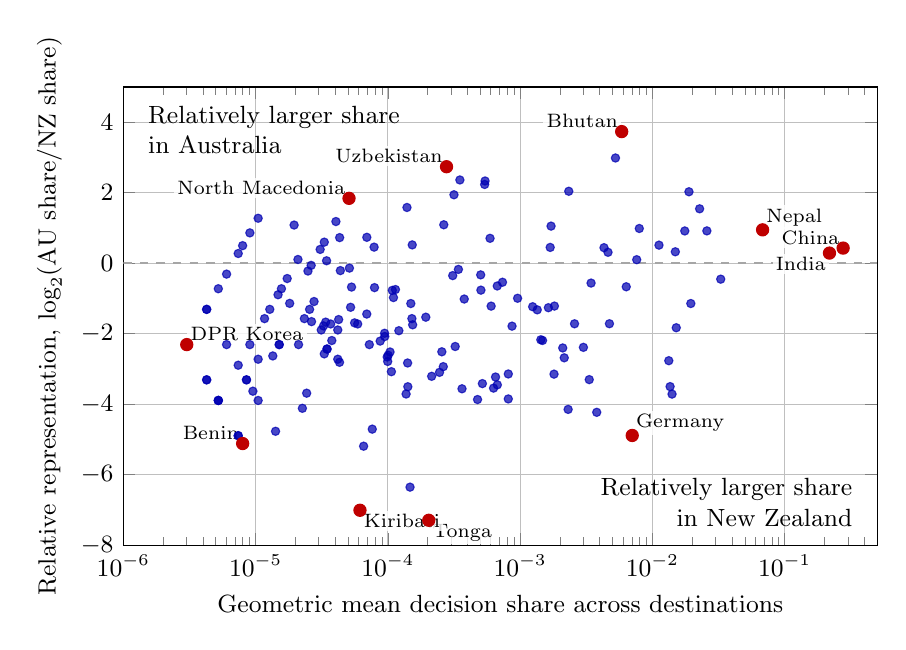
\begin{tikzpicture}
\begin{semilogxaxis}[
  width=0.92\textwidth,height=7.4cm,xmin=0.000001,xmax=0.5,ymin=-8,ymax=5,
  xlabel={Geometric mean decision share across destinations},
  ylabel={Relative representation, $\log_2(\mathrm{AU\ share}/\mathrm{NZ\ share})$},
  grid=major,tick label style={font=\small},label style={font=\small},
]
\addplot[gray!70,dashed,thick,domain=0.000001:0.5,forget plot] {0};
\addplot[only marks,mark=*,mark size=1.5pt,blue!70!black,opacity=0.72] coordinates {(0.000141653966367,-3.50519430713) (4.37550682435e-05,-0.210107824465) (3.46901105437e-05,-2.4351743801) (5.2297309368e-06,-3.89460599874) (0.000672788167152,-3.45151221433) (2.48984994571e-05,-0.222180656766) (0.000476757218423,-3.86823058331) (4.32310365463e-05,0.725980411715) (7.98854596071e-06,0.497711424041) (2.63224018092e-05,-0.0617159845726) (0.0227511072134,1.54366133588) (1.28101722872e-05,-1.30964349802) (3.46901105437e-05,-2.4351743801) (0.000363682573553,-3.56340009026) (1.04594618736e-05,-2.7246809973) (7.98854596071e-06,-5.11699842007) (4.27005742907e-06,-3.30964349802) (0.00586090465273,3.73392724357) (0.000106409282809,-3.07831795191) (9.05815969244e-06,0.860281503426) (0.000139546626609,1.58112743223) (0.00379622514813,-4.2310515294) (0.000264864058994,1.09028710887) (4.18378474944e-05,-1.89460599874) (3.07918220193e-05,0.390796220125) (4.27005742907e-06,-1.30964349802) (0.00461783267486,0.309592564005) (9.48106612709e-05,-2.08016165189) (0.00634508838478,-0.668797070514) (2.25950200825e-05,-4.11699842007) (0.00230697731626,-4.14828579265) (0.276698921953,0.428974440983) (0.0112174823151,0.512535523046) (0.000592461812698,0.705953357035) (0.00333170392898,-3.30317192979) (5.2297309368e-06,-3.89460599874) (4.18378474944e-05,-2.7246809973) (2.33880677574e-05,-1.57267790385) (0.000214440226424,-3.20911662206) (3.01938656415e-06,-2.30964349802) (5.9167651347e-05,-1.7246809973) (0.000629887748839,-3.54410875165) (7.39595641838e-06,0.275319002705) (2.09189237472e-05,0.105394001263) (2.43430727219e-05,-3.68815512127) (0.000518456017399,-3.41655870193) (0.000505492565456,-0.764482005353) (2.76731349651e-05,-1.08725107668) (1.81163193849e-05,-1.13971849657) (2.64950095722e-05,-1.65756680144) (1.50969328207e-05,-2.30964349802) (0.000152022440423,-1.57267790385) (0.00215574685597,-2.68443340729) (0.000256007659971,-2.51365739004) (0.00300922432395,-2.38780256094) (2.1135705949e-05,-2.30964349802) (0.00703969961243,-4.88803794833) (0.000735888372167,-0.540256426158) (5.2297309368e-05,-1.25074980896) (8.54011485813e-06,-3.30964349802) (6.93802210875e-05,0.734750621342) (6.0387731283e-06,-2.30964349802) (7.39595641838e-06,-4.89460599874) (1.50969328207e-05,-2.30964349802) (4.24865349764e-05,-1.59915011521) (0.000141105855189,-2.83159620121) (3.26596592325e-05,-1.77912878132) (0.218123454103,0.287010314115) (0.0175772120366,0.915047306857) (0.00343930794191,-0.563890825627) (0.000154077494666,-1.74776461041) (0.000245927135783,-3.09691417403) (9.8905075578e-05,-2.66111586852) (0.00180445422476,-3.14756416976) (3.30757226202e-05,-2.57267790385) (0.0140787219025,-3.71394426005) (0.000503468563072,-0.331273513988) (0.000378087002036,-1.01686174879) (0.00525936232302,2.98530775763) (6.15836440387e-05,-7.01008321616) (0.00163628188384,-1.26258469322) (7.93127965992e-05,-0.692972137568) (0.00143411008723,-2.17300880599) (3.7712126099e-05,-2.1941662806) (0.000350535045646,2.36155140035) (3.13783856208e-05,-1.89460599874) (1.41621783255e-05,-4.76907511665) (7.39595641838e-06,-2.89460599874) (5.31617862695e-05,-0.677375282517) (4.31254660919e-05,-2.81214383855) (1.04594618736e-05,1.2753190027) (7.87359686049e-05,0.455891248347) (0.0149093395146,0.324220515401) (0.000309453981442,-0.351871733405) (8.54011485813e-06,-3.30964349802) (1.73450552719e-05,-0.4351743801) (7.39595641838e-06,-4.89460599874) (0.000539541652878,2.23411988553) (0.00147826650004,-2.19180700772) (5.2297309368e-06,-3.89460599874) (0.00171372465682,1.05247368699) (6.93144889826e-05,-1.44291002888) (3.44263035932e-05,0.0688681252375) (0.00473401395397,-1.71754357725) (3.38925301238e-05,-1.6722135774) (5.12406891488e-05,-0.139718496574) (0.0681049885097,0.946615789339) (0.000651998758886,-3.22934186993) (6.0387731283e-06,-0.309643498016) (4.27005742907e-06,-1.30964349802) (0.00430725838328,0.440378248975) (5.08836068253e-05,1.84010362149) (0.00181702860239,-1.21642467006) (0.00060390750594,-1.2178510221) (0.018904449687,2.02676293508) (0.000103894981327,-2.51909686365) (0.00124430968141,-1.23538894332) (0.000114179131937,-0.746707303625) (0.000957197926235,-0.994910904533) (0.0195278615368,-1.1439567997) (0.000193711944756,-1.53203591935) (0.000341577905424,-0.175787751281) (0.0151538460548,-1.83121345426) (0.000110279968392,-0.975224458946) (0.00210034528155,-2.40502876385) (0.000108067046696,-0.771223583232) (1.47919128368e-05,-0.894605998737) (1.04594618736e-05,-3.89460599874) (0.000147177674433,-6.35403761737) (0.00233220787832,2.04110186929) (4.27005742907e-06,-3.30964349802) (3.30757226202e-05,0.597247097592) (1.95678613905e-05,1.08267392476) (4.05093216467e-05,1.18220959831) (0.00796326328856,0.984780795069) (0.000121152297998,-1.9153645589) (1.56891928104e-05,-0.724680997295) (0.000323017920302,-2.36358230513) (1.16940338787e-05,-1.57267790385) (0.00134718789275,-1.32336177926) (2.56203445744e-05,-1.30964349802) (0.000814227288091,-3.14328511159) (0.0328580153385,-0.452828809462) (5.60826163102e-05,-1.69297213757) (9.4521750509e-05,-1.98771540313) (9.54813867922e-06,-3.6315715929) (0.000868828155925,-1.78608154196) (0.000814003322391,-3.85135280078) (0.000100595883108,-2.61220626804) (0.00761294718517,0.0995302185157) (9.05815969244e-06,-2.30964349802) (0.0133039126569,-2.76645733307) (0.000262530409461,-2.93524798323) (5.2297309368e-06,-0.724680997295) (0.000203892447679,-7.29453660563) (3.69797820919e-05,-1.7246809973) (1.35031072156e-05,-2.6315715929) (6.55978669288e-05,-5.19228654738) (0.00067177110207,-0.646071162599) (0.000316214979427,1.94144435632) (8.75101364869e-05,-2.21010782447) (0.000543187558972,2.33260880606) (0.0025787187574,-1.71916399233) (0.000149207807223,-1.14458425175) (0.0136127669495,-3.50138146778) (7.62656643107e-05,-4.70819287451) (0.000277783563902,2.7374804141) (0.000137440141529,-3.71174194159) (9.97769070694e-05,-2.78769079482) (0.025818350606,0.916798854639) (7.24652775396e-05,-2.30964349802) (0.000152919335759,0.519244585591) (0.00168818544417,0.447975206314)};
\addplot[only marks,mark=*,mark size=2.2pt,red!75!black] coordinates {(0.276698921953,0.428974440983) (0.218123454103,0.287010314115) (0.0681049885097,0.946615789339) (0.00586090465273,3.73392724357) (0.00703969961243,-4.88803794833) (0.000203892447679,-7.29453660563) (5.08836068253e-05,1.84010362149) (6.15836440387e-05,-7.01008321616) (7.98854596071e-06,-5.11699842007) (0.000277783563902,2.7374804141) (3.01938656415e-06,-2.30964349802)};
\node[font=\small,align=left,anchor=north west] at (rel axis cs:0.02,0.98) {Relatively larger share\\in Australia};
\node[font=\small,align=right,anchor=south east] at (rel axis cs:0.98,0.02) {Relatively larger share\\in New Zealand};
\node[font=\scriptsize,anchor=south east,fill=white,fill opacity=0.82,text opacity=1,inner sep=1.2pt] at (axis cs:0.276698921953,0.428974440983) {China};
\node[font=\scriptsize,anchor=north east,fill=white,fill opacity=0.82,text opacity=1,inner sep=1.2pt] at (axis cs:0.218123454103,0.287010314115) {India};
\node[font=\scriptsize,anchor=south west,fill=white,fill opacity=0.82,text opacity=1,inner sep=1.2pt] at (axis cs:0.0681049885097,0.946615789339) {Nepal};
\node[font=\scriptsize,anchor=south east,fill=white,fill opacity=0.82,text opacity=1,inner sep=1.2pt] at (axis cs:0.00586090465273,3.73392724357) {Bhutan};
\node[font=\scriptsize,anchor=south west,fill=white,fill opacity=0.82,text opacity=1,inner sep=1.2pt] at (axis cs:0.00703969961243,-4.88803794833) {Germany};
\node[font=\scriptsize,anchor=north west,fill=white,fill opacity=0.82,text opacity=1,inner sep=1.2pt] at (axis cs:0.000203892447679,-7.29453660563) {Tonga};
\node[font=\scriptsize,anchor=south east,fill=white,fill opacity=0.82,text opacity=1,inner sep=1.2pt] at (axis cs:5.08836068253e-05,1.84010362149) {North Macedonia};
\node[font=\scriptsize,anchor=north west,fill=white,fill opacity=0.82,text opacity=1,inner sep=1.2pt] at (axis cs:6.15836440387e-05,-7.01008321616) {Kiribati};
\node[font=\scriptsize,anchor=south east,fill=white,fill opacity=0.82,text opacity=1,inner sep=1.2pt] at (axis cs:7.98854596071e-06,-5.11699842007) {Benin};
\node[font=\scriptsize,anchor=south east,fill=white,fill opacity=0.82,text opacity=1,inner sep=1.2pt] at (axis cs:0.000277783563902,2.7374804141) {Uzbekistan};
\node[font=\scriptsize,anchor=south west,fill=white,fill opacity=0.82,text opacity=1,inner sep=1.2pt] at (axis cs:3.01938656415e-06,-2.30964349802) {DPR Korea};
\end{semilogxaxis}
\end{tikzpicture}

\caption{Relative representation of 173 origins observed in both destinations. Horizontal position is the geometric mean of the origin's Australian and New Zealand decision shares and is shown on a logarithmic scale. Vertical position is the base-2 logarithm of the Australian share divided by the New Zealand share. Zero denotes equal shares, $+1$ denotes an Australian share twice the New Zealand share, and $-1$ denotes a New Zealand share twice the Australian share. Red points identify reproducibly selected high-share origins, relative-share extrema, upper and lower boundaries in the left tail of the distribution, and the leftmost origin.}
\label{fig:relative-origin-representation}
\end{figure}

\subsection{Supporting Result: Annual Variation}

Annual destination summaries varied in scale and in decision-weighted and equally weighted rates (Table~\ref{tab:annual-destination-summary}). Australia recorded 159,002 to 231,156 decisions per year, compared with 18,013 to 48,773 in New Zealand. The aggregate approval rate ranged from 81.6\% to 90.7\% in Australia and from 75.6\% to 90.6\% in New Zealand. Median origin rates were 98.6\% to 98.9\% in Australia and 85.7\% to 98.0\% in New Zealand. The clearest change in direction occurred in 2022. New Zealand's decision-weighted aggregate approval rate was 90.6\%, compared with 88.9\% for Australia, while the equally weighted mean across matched origins gave an Australian-minus-New Zealand difference of 5.3 points (95\% CI 0.6 to 9.9). National decision-weighted rates and origin-weighted comparisons therefore answered different questions.

On year-specific matched-origin support, the equally weighted mean difference between the Australian and New Zealand rates was positive in every year: 5.3 points in 2022, 13.1 in 2023, 12.7 in 2024, and 14.8 in 2025 (Figure~\ref{fig:annual-matched-differences}). The corresponding median differences were 0.0, 4.1, 2.9, and 0.7 points. These origin-weighted summaries differ from the decision-weighted matched-support differences used in the decomposition. The rate component remained positive and the composition component remained negative throughout 2022--2025 (Figure~\ref{fig:annual-decomposition-components}). The observed matched-support difference was $-1.7$ points in 2022 (95\% CI $-6.6$ to 3.0), 0.6 points in 2023 ($-6.5$ to 5.0), 11.9 points in 2024 ($-0.9$ to 20.6), and 6.3 points in 2025 (0.4 to 14.3). The common-weight rate component was 5.0, 8.9, 13.5, and 9.2 points, respectively. The composition component offset those differences by $-6.7$, $-8.4$, $-1.5$, and $-2.9$ points. Its interval excluded zero in 2022 and 2023 but not in 2024 or 2025. Restricting the comparison to the same 118 origins observed in both destinations in all four years reproduced these component estimates to one decimal place. Annual changes in the observed difference therefore reflected changes in both origin-specific approval rates and the distribution of recorded decisions across origins.

% Generated by scripts/generate_article_temporal_sensitivity_outputs.py. Do not edit.
\begin{table}
\caption{Annual destination scale and approval-rate summaries}
\label{tab:annual-destination-summary}
\centering
\small
\begin{tabular*}{\textwidth}{@{\extracolsep{\fill}}lrrrrrr@{}}
\toprule
Year & AU decisions & NZ decisions & AU aggregate & NZ aggregate & AU median & NZ median \\
\midrule
2022 & 161,867 & 18,013 & 88.9\% & 90.6\% & 98.8\% & 98.0\% \\
2023 & 231,156 & 40,460 & 81.6\% & 80.9\% & 98.7\% & 85.7\% \\
2024 & 185,399 & 48,773 & 87.6\% & 75.6\% & 98.6\% & 88.5\% \\
2025 & 159,002 & 41,500 & 90.7\% & 84.4\% & 98.9\% & 91.7\% \\
\bottomrule
\end{tabular*}
\parbox{0.96\textwidth}{\scriptsize Notes: Aggregate rates weight recorded decisions. Median rates weight represented origins equally. All rates use the common two-outcome decision denominator.}
\end{table}


\begin{figure}
\centering
% Generated by scripts/generate_article_temporal_sensitivity_outputs.py. Do not edit.
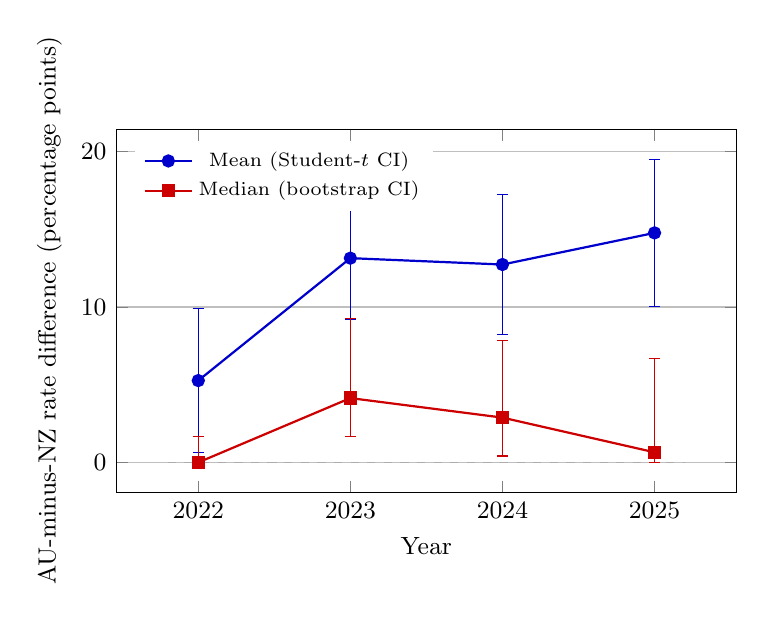
\begin{tikzpicture}
\begin{axis}[width=0.78\textwidth,height=6.2cm,xtick={{2022,2023,2024,2025}},xticklabels={{2022,2023,2024,2025}},xlabel={Year},ylabel={AU-minus-NZ rate difference (percentage points)},ymajorgrids=true,legend style={font=\scriptsize,draw=none,at={{(0.03,0.97)}},anchor=north west},label style={font=\small},tick label style={font=\small}]
\addplot[gray!65,dashed,domain=2021.8:2025.2,forget plot] {0};
\addplot+[blue!80!black,thick,mark=*,error bars/.cd,y dir=both,y explicit] coordinates {(2022,5.26713043495) += (0,4.62154495928) -= (0,4.62154495928) (2023,13.1435706402) += (0,3.92634428999) -= (0,3.92634428999) (2024,12.7334924088) += (0,4.50735861076) -= (0,4.50735861076) (2025,14.7680201261) += (0,4.72986999035) -= (0,4.72986999035)};\addlegendentry{Mean (Student-$t$ CI)}
\addplot+[red!80!black,thick,mark=square*,error bars/.cd,y dir=both,y explicit] coordinates {(2022,0) += (0,1.67301945586) -= (0,0) (2023,4.13992641082) += (0,5.12855217521) -= (0,2.46561913534) (2024,2.88461538462) += (0,4.93555255585) -= (0,2.46918511755) (2025,0.652379260641) += (0,6.04812223288) -= (0,0.652379260641)};\addlegendentry{Median (bootstrap CI)}
\end{axis}
\end{tikzpicture}

\caption{Annual equally weighted matched-origin Australian-minus-New Zealand approval-rate differences. Points show the mean with $t$-based 95\% intervals and the median with fixed-seed percentile-bootstrap 95\% intervals on year-specific matched support. Each observed matched origin receives equal weight. These estimates are distinct from the decision-weighted observed gaps in Figure~\ref{fig:annual-decomposition-components}.}
\label{fig:annual-matched-differences}
\end{figure}

\begin{figure}
\centering
% Generated by scripts/generate_article_b_decomposition_outputs.py. Do not edit.
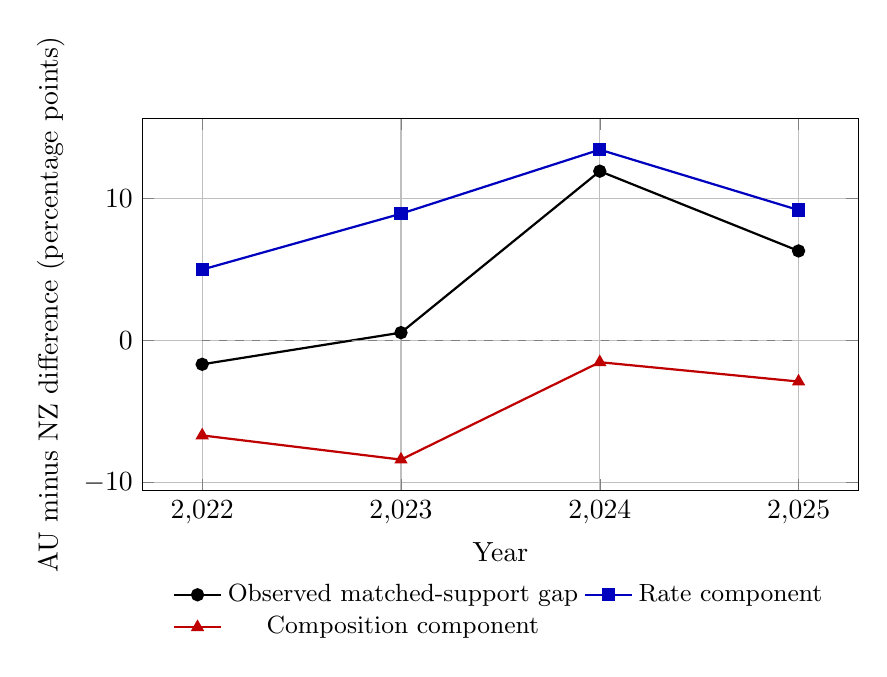
\begin{tikzpicture}
\begin{axis}[width=0.88\textwidth,height=0.52\textwidth,xlabel={Year},ylabel={AU minus NZ difference (percentage points)},xtick={2022,2023,2024,2025},grid=major,legend style={font=\small,draw=none,at={(0.5,-0.22)},anchor=north,legend columns=2}]
\addplot[black,thick,mark=*] coordinates {(2022,-1.66263406) (2023,0.56675021) (2024,11.93753105) (2025,6.32031392)};
\addlegendentry{Observed matched-support gap}
\addplot[blue!75!black,thick,mark=square*] coordinates {(2022,5.00790917) (2023,8.94207643) (2024,13.45213767) (2025,9.19777630)};
\addlegendentry{Rate component}
\addplot[red!75!black,thick,mark=triangle*] coordinates {(2022,-6.67054323) (2023,-8.37532622) (2024,-1.51460662) (2025,-2.87746237)};
\addlegendentry{Composition component}
\addplot[gray,dashed] coordinates {(2022,0) (2025,0)};
\end{axis}
\end{tikzpicture}

\caption{Annual symmetric decomposition of the observed Australian-minus-New Zealand approval-rate difference on year-specific matched-origin support. The rate and composition components sum to the observed gap in each year. Components are descriptive accounting quantities, not causal effects.}
\label{fig:annual-decomposition-components}
\end{figure}

\subsection{Supporting Country--Year Comparison}

The country--year model provided supporting evidence that the Australian--New Zealand difference remained after accounting for origin and year. It retained 525 matched country--year pairs from 145 origins, representing 884,997 decisions. The standardised approval probabilities were 87.1\% for Australia and 77.4\% for New Zealand, giving an Australian-minus-New Zealand contrast of 9.8 percentage points (95\% CI 6.6 to 12.9). The odds ratio for Australia relative to New Zealand was 2.50 (95\% CI 1.84 to 3.39; $p<0.001$). The model converged without fitting warnings or unresolved separation, but its Pearson dispersion ratio was 19.28, indicating substantial residual heterogeneity. The adjusted contrast therefore corroborates the positive common-weight rate component but does not replace the weighting and decomposition results or identify a causal destination effect.

\section{Discussion}

The preceding study found that the average recorded approval rate was higher for Australia than for New Zealand. This study asked whether the difference could be accounted for by how decisions were distributed across origins and years. The main answer is no: assigning both destinations the same average origin distribution increased the Australian-minus-New Zealand difference from 5.3 to 10.9 percentage points, while the composition component was $-5.6$ points. The 2022 results provide a simple example of why weighting still matters. New Zealand had the higher decision-weighted aggregate rate, while the equally weighted matched-origin comparison favoured Australia. These are descriptive accounting comparisons rather than causal effects. Table~\ref{tab:discussion-question-answers} summarises the main answer and the supporting findings.

\begin{table}
\caption{Questions answered by this study. Australian-minus-New Zealand differences are positive when the Australian recorded approval rate is higher.}
\label{tab:discussion-question-answers}
\centering
\small
\begin{tabular*}{\textwidth}{@{\extracolsep{\fill}}p{0.31\textwidth}p{0.10\textwidth}p{0.48\textwidth}@{}}
\toprule
Question & Answer & Explanation \\
\midrule
Is Australia's higher recorded rate explained by origins with higher observed Australian rates accounting for larger shares of its decisions? & No. & With the same average origin distribution, the standardised rates were 88.5\% for Australia and 77.6\% for New Zealand. The 10.9-point difference was larger than the 5.3-point difference under the origin shares observed in the data. \\
\midrule
Are decisions distributed similarly across origins? & No. & Australian decisions were more concentrated. The largest origin accounted for 32.1\% of Australian decisions and 23.8\% of New Zealand decisions. The top five accounted for 73.4\% and 58.2\%, respectively. \\
\midrule
Do the same origins tend to contribute large decision volumes in both destinations? & Yes. & Matched-origin shares had a strong rank association (Spearman $\rho=0.858$), although the share of individual origins differed. \\
\midrule
Does the weighting rule change the comparison? & Yes. & The pooled difference ranged from 5.3 points under the observed destination-specific shares to 16.3 points when every matched origin received equal weight. In 2022, changing the weights also changed the direction. \\
\midrule
Did origin composition produce Australia's higher average rate? & No. & The composition component was $-5.6$ points. The distribution of recorded decisions across origins reduced the pooled Australian-minus-New Zealand difference. \\
\midrule
Was the pattern the same every year? & No. & The rate component calculated under the same origin shares was positive in every year, but its size and the observed decision-weighted gap varied from 2022 to 2025. \\
\midrule
Was the annual pattern caused only by origins entering or leaving the data? & No. & Following the same 118 origins across all four years reproduced the component estimates to one decimal place. \\
\midrule
Did Australia retain a higher average rate after accounting for origin and year? & Yes. & The adjusted difference was 9.8 points (95\% CI 6.6--12.9). Substantial residual heterogeneity remained, so the estimate did not represent every origin and year. \\
\bottomrule
\end{tabular*}
\end{table}


The composition findings explain why similar origin rankings do not imply comparable national summaries. Many of the same origins contributed relatively large decision volumes in both destinations, but Australian decisions were more concentrated and individual origin shares differed. Correlation describes the ordering of shares, whereas concentration describes how strongly total volume accumulates among the largest origins. A national approval rate combines these shares with origin-specific outcomes. Observed-share, common-weight, and equal-origin estimates therefore describe different populations or weighting rules rather than competing estimates of one quantity.

The decomposition clarifies the role of composition in this study. The rate component was positive and the composition component negative in the pooled analysis and in every year. The observed distribution of decisions therefore offset part of the positive average rate difference instead of producing it. The size of that offset changed across years, while the balanced-panel analysis showed that the pattern was not simply caused by origins entering or leaving the matched sample. The country--year model supported the same average direction after accounting for origin and year, but its substantial residual dispersion confirmed that one adjusted contrast did not represent every origin or year.

These findings extend the origin--destination perspective used in research on international student mobility \cite{PerkinsNeumayer2014,Weber2023}. For visa statistics, an origin--destination relationship includes both the recorded outcome within an origin and the weight that the origin receives in a destination's published data. Comparisons should therefore state the administrative population, decision denominator, origin support, period, and weighting rule. Missing origins should also remain distinguishable from observed zero decisions. Making these choices explicit prevents a difference in record composition from being mistaken for a difference in within-origin outcomes.

\section{Limitations}

The main limitation is the short observation period. Four years of data are sufficient to show that the observed difference, the rate component, and the composition component varied from year to year. They are not sufficient to establish a permanent relationship, distinguish long-term trends from temporary changes, or identify the effects of particular policy or administrative events. The 2022--2025 period may also reflect conditions specific to those years. The annual findings should therefore be interpreted as evidence about this period rather than as a forecast of future approval rates or origin distributions. Australia and New Zealand publish recurring decision data, so the analysis can be repeated after several additional years become available. Such updates would show whether the observed pattern persists, weakens, or changes direction. They would also permit more informative analysis of temporal changes, provided that the published populations, categories, and definitions remain sufficiently comparable.

The Australian and New Zealand records describe similar rather than identical administrative populations. Applying the same origin distribution improves comparability of the weighting but cannot remove differences in visa categories, eligibility rules, or source coverage.

The records are aggregated by applicant origin and contain no individual characteristics. The findings therefore apply to groups of recorded decisions and cannot be interpreted as individual approval probabilities. Paired analyses also include only origins with positive observed decision totals in both destinations. Origins absent from one source were treated as unobserved rather than assigned zero decisions. The decomposition consequently describes the matched support, although the decision-count threshold and balanced-panel analyses indicate that the main result was not driven by sparse origins or by origins entering and leaving the annual matched samples.

Finally, substantial heterogeneity remained after adjustment for origin and year. The country--year model had a Pearson dispersion ratio of 19.28, showing that a single average destination contrast did not represent every origin and year. Cluster-robust uncertainty addresses dependence among repeated observations from the same origin, but it does not remove this heterogeneity or establish a common effect. Longer time series and more closely aligned applicant-level data would be required to investigate the mechanisms behind the observed differences.

\section{Conclusion}

This study asked whether Australia's higher average recorded approval rate could be accounted for by origins with higher observed Australian rates contributing larger shares of its decisions. It could not. Under each destination's observed origin shares, the Australian-minus-New Zealand difference was 5.3 percentage points. Assigning both destinations the same average origin distribution increased the difference to 10.9 points, while the $-5.6$-point composition component showed that the observed distribution reduced rather than produced the positive average difference. Weighting still affected its magnitude, and in 2022 the weighting rule changed the direction of the comparison. National approval rates therefore cannot be interpreted without specifying which origins contribute decisions, how those decisions are weighted, and which period is being described.

This article completes a three-part research sequence. The first article showed that recorded New Zealand approval rates varied across applicant origins and were associated with application volume and with regional, economic, development, and health characteristics \cite{Kaplan2026NZVisaApproval}. The second compared the same published origins across Australia and New Zealand, finding a positive average Australian-minus-New Zealand difference under its study definitions alongside substantial variation and some differences in the opposite direction \cite{Kaplan2026AUNZDecisionOutcomes}. This third article shows that the distribution of decisions across origins and years altered the size of that average difference and partly offset it, but did not account for it.

Together, the three studies provide a broader account of published student-visa approval statistics. Recorded rates vary across origins within a destination, the same origin can have different recorded rates across destinations, and national summaries depend on how decision volume is distributed across origins and time. Approval rates are therefore neither fixed attributes of origin countries nor context-free measures of destinations. They are aggregate outcomes for particular origin--destination populations, observed during a specified period and summarised under a particular weighting rule.

The analysis remains descriptive rather than causal. The three studies identify statistical structure but do not determine why origin-specific rates or origin distributions differ. Applicant demand, selection before application, institutional recruitment, visa-category coverage, policy, administrative practice, and unobserved applicant characteristics remain possible explanations that these aggregate records cannot separate. Additional years of comparable public data will allow the temporal pattern to be reassessed, while more closely aligned categories and applicant-level or case-level data would be required to investigate the mechanisms behind the observed origin--destination differences.

\bibliographystyle{splncs04}
\bibliography{bibliography}

\end{document}
